\documentclass[a4paper,10pt]{report}
\usepackage[utf8]{inputenc}
\usepackage[T1]{fontenc}
\usepackage{graphics}
\usepackage{graphicx}
\usepackage{eurosym}
\usepackage{fullpage}
\usepackage[francais]{babel}
\usepackage{subcaption}

\title{\textbf{Projet Njörd}\\ Topographie d'une zone \\ par communication avec 
une équipe de drones}
\author{AIGREAULT Clément - HENRIO Jordan - PHAM Chitin}

\begin{document}

  \maketitle

  \chapter*{Introduction}
    Nous vivons dans un monde où la technologie a atteint un point permettant 
de “donner vie” à des objets. Si bien qu’ils peuvent prendre des décisions, 
apprendre et communiquer. Une telle avancée permet des milliers d’applications 
aussi bien pour le divertissement, la domotique, l’industrie, ou encore 
l’assistance.
    
    Parfois l’homme peut être amené à devoir exécuter certaines missions sur 
des terrains dont il ne possède pas une connaissance exacte (comme par exemple 
une ville ayant subi une catastrophe naturelle). Ainsi un des problèmes majeurs 
des agents de sécurité est de connaître exactement la situation afin de mettre 
en place une stratégie d’approche. Des pertes humaines ne sont pas un risque à 
prendre, alors un intermédiaire devient nécessaire. 

    Grâce à l'avancée de la robotique, de l'intelligence artificielle et de nos 
moyens de communication sans fil, la création d’une équipe de robots permettant 
l’analyse d’un lieu peut être d’une très grande utilité dans ce genre de 
situation. Des pertes matérielles ne sont pas aussi grave que des pertes 
humaines. 

  C'est pourquoi nous avons choisi, dans le cadre de notre projet de fin 
d'études, de créer une équipe de drones volants qui communiquent ensemble par 
l'implémentation d'un serveur central qui reçoit des informations de la part 
des drones et qui dessine la topographie de la zone analysée. Ce rapport a pour 
but de présenter le développement et les choix technologiques de ce projet. Il 
explique les calculs réalisés pour le choix des composants, les erreurs que 
nous avons faites et présente les résultats obtenus pendant les phases de tests.
  
  \tableofcontents
  
  \chapter{Serveur}
    Le but de ce chapitre est de présenter le serveur mis en place. Dans un 
premier temps nous expliquons le modèle de réseau utilisé pour la communication 
entre les drones et le serveur, puis le fonctionnement interne du serveur. Dans 
une deuxième partie nous abordons, la manière dont nous avons implémenté cela.

    \section{Principe de fonctionnement}
      \subsection{Modèle du réseau}
	Pour réaliser notre application nous avons choisi de mettre en place un 
modèle de communication basé sur un réseau étoilé. Le serveur représente le 
noyau du modèle et les branches sont représentées par les drones (voir 
Figure \ref{network_schema}). Ainsi l'objectif du serveur est de dessiner la 
topographie de la zone étudiée à l'aide des données récoltées par l'équipe de 
drones. Bien que les drones se doivent d'être indépendants, il est important de 
toujours en garder le contrôle. Ainsi, le serveur a aussi la possibilité 
d'envoyer des ordres aux drones suivant certaines situations.

	\begin{figure}[htbp]
	  \centering
	  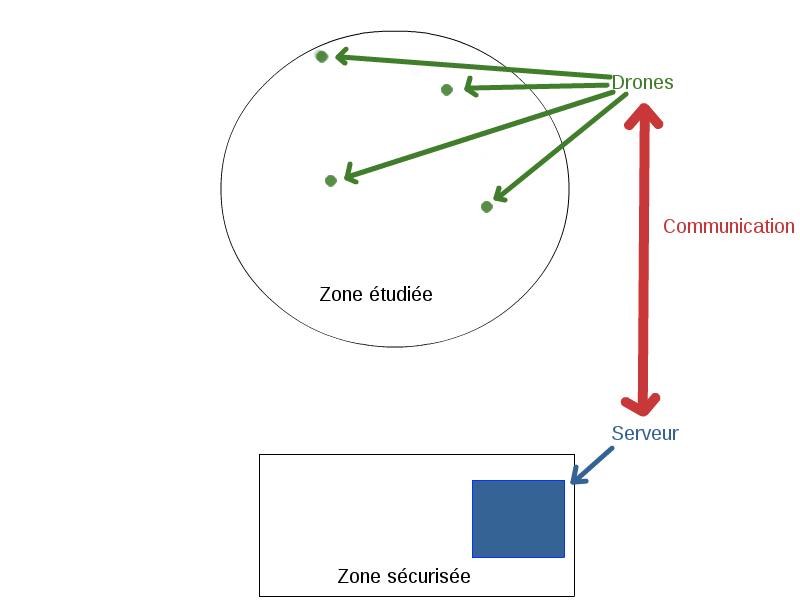
\includegraphics[scale=0.4]{img/projet_schema.png}
	  \caption{Schéma du réseau}
	  \label{network_schema}
	\end{figure}
	
	\newpage
	
	Nous avons choisi ce modèle car il répond à nos besoins et qu'il est 
plus simple à mettre en place qu'un réseau maillé par exemple. Chaque 
drone peut communiquer avec le serveur, mais pas les autres drones. Et le 
serveur connait l'ensemble des drones utilisés dans l'application et peut 
donc communiquer avec eux. Aussi, si l'un des drones venait à tomber en panne 
durant une analyse, cela n'empêcherait pas le bon déroulement de l'application 
puisque le serveur pourrait continuer de communiquer avec le reste des drones, 
contrairement à une topologie en anneau par exemple (qui au passage 
augmenterait la latence de réception des données).
      
      \subsection{Fonctionnement interne du serveur}
	En ce qui concerne le fonctionnement interne du serveur nous avons 
pensé qu'il serait plus judicieux de le découper en plusieurs entités, où 
chacune d'elle serait associée à une tâche particulière. Ainsi, nous avons 
effectué le découpage suivant :

\begin{itemize}
  \item Communication
  \item Sauvegarde/Chargement des données
  \item Topographie/Décision d'ordre
\end{itemize}

	Le serveur est donc constitué de trois tâches qui tournent en 
concurrence à "l'infinie". En fait, si nous avions fait une seule et unique 
tâche nous risquerions de perdre des données. En effet, le temps que le serveur 
traite les informations qu'il a reçues, les drones continuent de lui envoyer 
des données. Mais si le serveur n'écoute pas à ce moment là, alors ces données 
sont perdues.	

	\begin{figure}[htbp]
	  \centering
	  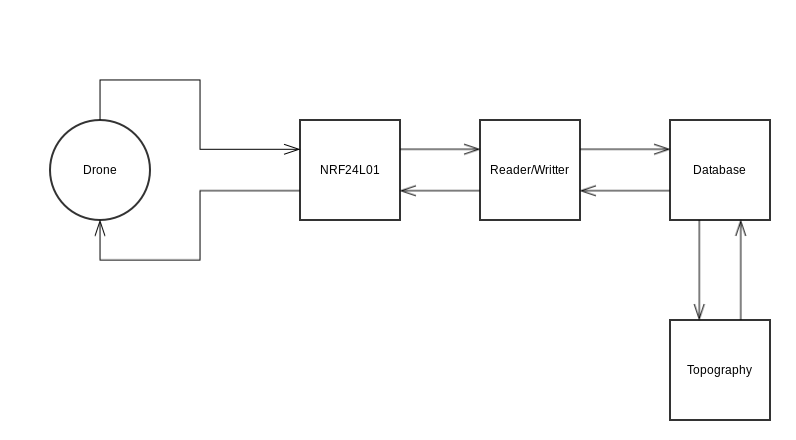
\includegraphics[scale=0.45]{img/server_model.png}
	  \caption{Transitions des données}
	  \label{server_model}
	\end{figure}
	
	La première tâche, \textit{Communication} (nommée \textit{NRF24L01} sur 
la Figure \ref{server_model}, en référence au composant utilisé pour la 
communication), se charge de lire les messages envoyés par les différents 
drones et de les réécrire sur le port série du serveur. En effet, une partie du 
serveur est constitué d'un montage à base d'\textit{Arduino} et c'est notre 
seul moyen de faire passer les données du micro-contrôleur (voir section 2.1.1) 
vers le serveur. Cette même tâche se charge dans un deuxième temps de lire le 
port série, afin de vérifier s'il y a des ordres à envoyer aux drones. Si c'est 
le cas elle se charge de les communiquer aux drones concernés.

	La deuxième tâche, \textit{Sauvegarde/Chargement des données} (nommée 
\textit{Reader/Writer} sur la Figure \ref{server_model}), lit le port série du 
serveur et enregistre chaque message dans une base de données. Dans un deuxième 
temps elle accède au contenu de la base de données, afin de vérifier si des 
ordres doivent être envoyés. Si c'est le cas elle les écrit sur le port série 
afin de les transmettre à la première tâche.

	La troisième et dernière tâche, \textit{Topographie/Décision d'ordre} 
(nommée \textit{Topography} sur la Figure \ref{server_model}), récupère les 
entrées de la base de données (qui se comporte comme une pile) et les insère 
dans une matrice. Cette matrice représente la zone étudiée en vue de dessus, 
avec chacune de ses composantes représentant l'altitude aux cordonnées 
correspondantes aux indices de la composante. Ainsi, si $M_{1, 1} = 150$ (avec 
$M$ la matrice représentant la zone) cela signifie qu'au point $(1, 1)$ de la 
zone un drone a mesuré une altitude de 150 centimètres. À chaque fois 
qu'une donnée est insérée dans la matrice, cette tâche se charge de dessiner 
le nouveau contenu à l'écran. Ce qui permet à l'utilisateur de suivre en 
direct l'évolution de l'analyse, et ce, de manière graphique. Dans un deuxième 
temps cette tâche analyse si un ordre doit être envoyé. Cela dépend de 
plusieurs paramètres. Par exemple, si une zone de la carte n'a pas encore été 
dévoilée le serveur peut demander à un drone de s'y rendre pour y récolter des 
informations. Ou si un drone n'a plus beaucoup de batterie, le serveur peut lui 
demander de revenir dans la zone sécurisée afin que l'utilisateur le recharge. 
Si cette troisième tâche détermine qu'un ordre doit être envoyé, alors elle 
l'écrit dans la base de données afin de le faire remonter à la seconde tâche.

	Maintenant que nous en savons un peu plus sur le principe de 
fonctionnement, nous pouvons présenter la manière dont nous avons implémenté 
cela.
    
    \section{Implémentation}
      La première tâche est constituée d'une partie matérielle et logicielle. 
La partie matérielle est un simple montage formé par une carte Arduino et un 
transmetteur/récepteur radio (voir Figure \ref{montage_serveur}).

	\begin{figure}[htbp]
	  \centering
	  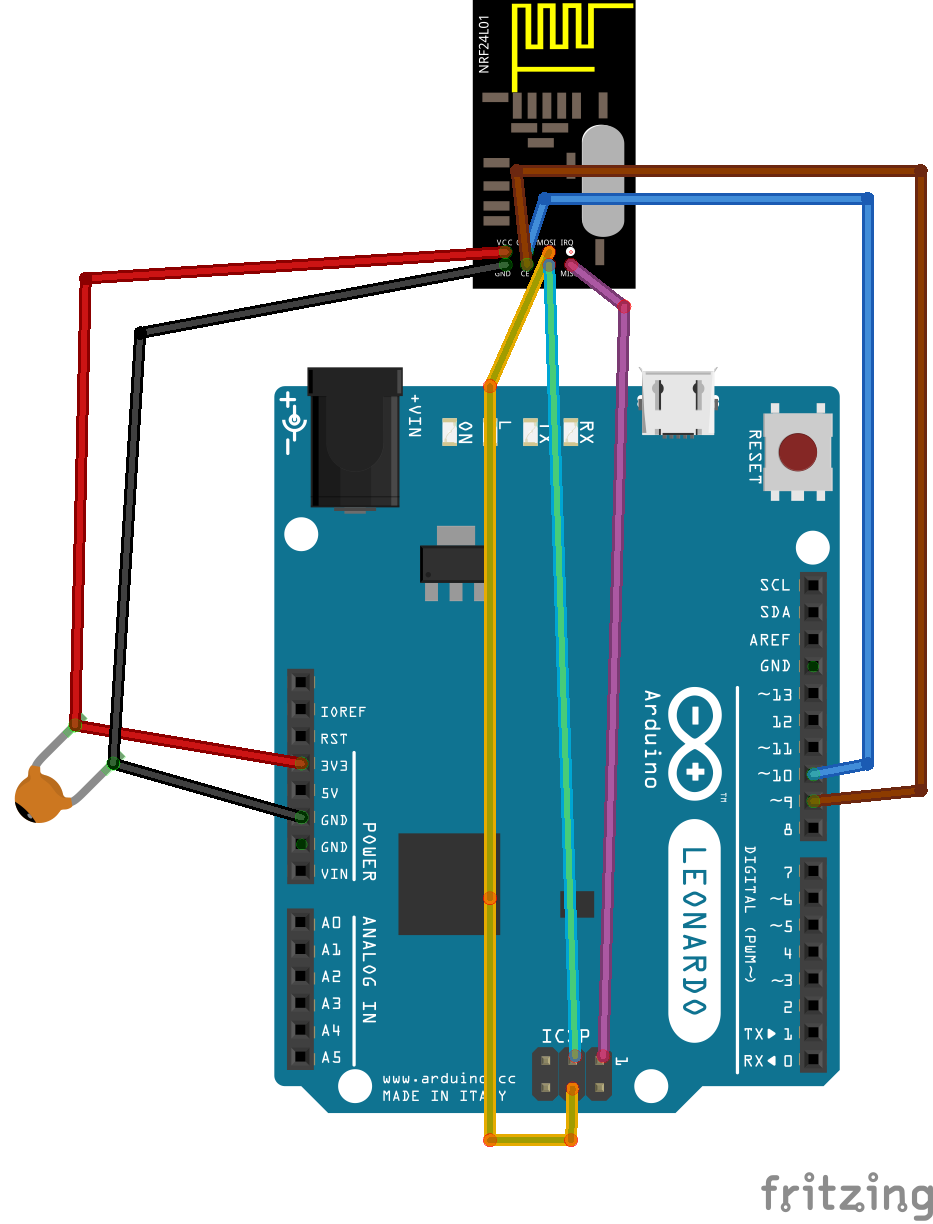
\includegraphics[scale=0.8]{img/montage_serveur.png}
	  \caption{Montage matériel du serveur}
	  \label{montage_serveur}
	\end{figure}
	
      Puisque cette tâche utilise un montage à base d'Arduino, la partie 
logicielle de cette tâche est codée dans le langage d'Arduino. Ce programme se 
contente de parcourir l'ensemble des adresses des drones connus et de lire les 
messages reçus. Un message est représenté par un tableau de la forme indiquée 
par la Figure \ref{message_drone}.

	\begin{figure}
	  \begin{center}
	    \begin{tabular}{|c|c|c|c|c|c|c|c|c|c|c|}
	      \hline
	      $d$ & $x$ & $y$ & $z$ & $s1$ & $s2$ & $s3$ & $s4$ & $s5$ & $s6$ & 
$e$ \\
	      \hline
	    \end{tabular}
	  \end{center}
	  \caption{Représentation d'un message de drone}
	  \label{message_drone}
	\end{figure}
	
	Avec :
	\begin{itemize}
	  \item $d$ : identifiant du drone
	  \item $x$ : position en abscisse
	  \item $y$ : position en ordonnée
	  \item $z$ : altitude du drone
	  \item $s1$ à $s6$ : valeurs des capteurs
	  \item $e$ : code d'état
	\end{itemize}

	La tâche se charge alors de recopier le contenu des tableaux, sur le 
port série afin de les communiquer à la deuxième tâche. Une fois l'ensemble des 
messages recopiés, elle lit le port série afin de voir si des ordres doivent 
être envoyés. Si c'est le cas, elle forme un tableau (représenté par la 
Figure \ref{message_serveur}) et le transmet au drone concerné.

	\begin{figure}
	  \begin{center}
	    \begin{tabular}{|c|c|c|c|c|}
	      \hline
	      $d$ & $x$ & $y$ & $z$ & $e$ \\
	      \hline
	    \end{tabular}
	  \end{center}
	  \caption{Représentation d'un ordre}
	  \label{message_serveur}
	\end{figure}
	
	Avec :
	\begin{itemize}
	  \item $d$ : identifiant du drone destinataire
	  \item $x$ : position cible en abscisse
	  \item $y$ : position cible en ordonnée
	  \item $z$ : altitude cible
	  \item $e$ : code supplémentaire
	\end{itemize}
	
	Que ce soit pour les messages ou pour les ordres, on peut remarquer 
qu'une valeur $e$ est présente dans la dernière case du tableau. Cette valeur 
additionnelle permet de communiquer une information supplémentaire dans un 
message. Par exemple, on peut imaginer qu'un drone envoie $e = 5$ ce qui 
pourrait signifier "Je n'ai plus de batterie". Dans ce cas le serveur sait 
interpréter le cas où $e = 5$ et construirait un ordre en conséquence.

	La deuxième tâche, quant à elle, est implémentée en 
\textit{Python}\cite{python}. Nous avons choisi ce langage, car nous n'avons 
pas besoin d'un langage puissant comme le \textit{C/C++} et il est moins 
gourmand que \textit{Java}. De plus, il possède une communauté énorme. Ainsi, 
il existe des bibliothèques pour tout et n'importe quoi. Le langage étant très 
simple de base, avec toutes ces bibliothèques il devient sûrement le langage le 
plus simple pour déployer de petites applications. Par exemple, il existe une 
bibliothèque pour accéder au port série de la machine, avec des fonctions très 
simples d'utilisation.

	Quand la deuxième tâche récupère un message elle doit l'insérer dans 
une base de données. Notre application ne nécessite pas la puissance du 
\textit{SQL}. En effet, tout ce que nous voulons faire c'est récupérer tout le 
contenu, entrée par entrée. Ainsi, nous n'avons pas besoin de faire des 
requêtes avec des entrées classées dans un certain ordre, ou alors des requêtes 
avec des conditions, etc. C'est pour cette raison que nous avons choisi 
d'utiliser une base de données \textit{Redis}\cite{redis}. C'est une base de 
données basée sur des ensembles "clé-valeur". Ainsi, dans notre application la 
zone étudiée (la clé) sera associée à une pile de messages (la valeur). Un 
autre point fort de notre choix d'implémentation est qu'il existe une 
bibliothèque pour la manipulation de Redis avec Python. 

      La troisième tâche est aussi implémentée en Python. Dans la section 
1.1.2 nous avons expliqué que nous représentons la zone étudiée par une 
matrice. Nous partons du principe que nous ne connaissons pas la taille de la 
zone. Ainsi, notre matrice doit être constamment redimensionnée. Il existe 
encore une bibliothèque très utile en Python, nommée 
\textit{Numpy}\cite{numpy}. C'est une bibliothèque scientifique qui propose 
divers fonctions implémentant des algorithmes connus pour le calcul 
scientifique, mais dans notre cas ce qui nous intéresse, ce sont les structures 
de données qu'elle propose. En effet, les matrices Numpy sont très puissantes, 
car elles disposent de divers méthodes pour leur manipulation et notamment des 
méthodes de redimensionnement dynamique.

      Aussi, cette tâche doit représenter graphiquement le contenu de la 
matrice. Numpy est très souvent couplé à une seconde bibliothèque nommée 
\textit{MatPlotLib}\cite{matplotlib}. Celle-ci permet de dessiner des 
graphiques à l'écran. Elle fonctionne très bien avec Numpy puisque ses méthodes 
s'attendent déjà à recevoir des objets venant de cette dernière.

      Maintenant que nous avons présenté le fonctionnement du serveur nous 
allons pouvoir vous présenter un exemple de résultat.

    \section{Résultat}
      La Figure \ref{exemple_topo} est une capture d'écran d'une topographie 
que 
nous avons obtenue par le biais du serveur.

	\begin{figure}[htbp]
	  \centering
	  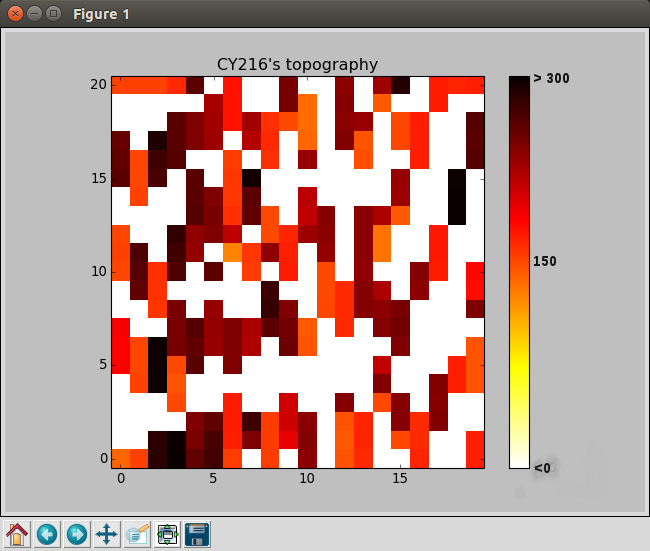
\includegraphics[scale=0.4]{img/topography_example.png}
	  \caption{Exemple de topographie}
	  \label{exemple_topo}
	\end{figure}
	
      On peut y voir un certain nombre d'éléments. Le plus visible est le 
graphique lui-même. Il représente la zone étudiée en vue de dessus. Ainsi à 
chaque coordonnée de la zone est associée une certaine hauteur. Le degré de 
cette hauteur est représenté par une couleur plus ou moins foncée. Plus cette 
couleur est foncée plus le point est élevé. Sur la droite du graphique se 
trouve sa légende. Elle indique la valeur en centimètres du degré de hauteur. 
On remarque donc que les points blancs représentent le sol, et que les points 
noirs représentent une hauteur de trois mètres. Cela est dû au fait que les 
capteurs ultrasons que nous utilisons pour les mesures ont une distance de 
mesure maximum. Mais le serveur lui peut fonctionner avec n'importe quelle 
valeur. Il ne dépend donc pas du matériel utilisé, mais seulement de la forme 
des messages reçus.

      Il faut noter que nous ne possédions pas de drone fonctionnel pour faire 
les essais du serveur. Ainsi l'exemple de topographie montré par la 
Figure \ref{exemple_topo} ne représente rien de spécial. Nous avons fournit des 
coordonnées aléatoires pour chaque point et nous avons fait varier les mesures 
du capteur en plaçant notre main devant et en jouant avec la distance.

      Dans tous les cas, lors de ces essais la réception et la représentation 
des messages se sont avérées fonctionnelles. Ainsi, si le serveur était utilisé 
avec un drone qui fournit sa véritable position et les valeurs renvoyées par 
ses capteurs, le serveur fournirait toujours les résultats attendus.

    \section{Envoi d'ordres}
      Toutefois, le serveur n'est pas encore totalement fonctionnel. Il reste 
l'envoi d'ordre à implémenter. La troisième tâche peut déterminer si une partie 
de la carte contient une zone encore non découverte. Ainsi, elle parcourt 
l'ensemble des drones et vérifie s'il existe un drone pour lequel un ordre n'a 
pas été donné (c'est-à-dire s'il existe un drone qui n'est pas en cours de 
déplacement vers une position cible). Si c'est le cas elle insère un ordre dans 
une deuxième pile Redis. La deuxième tâche lit le contenu de cette seconde 
pile. Si elle n'est pas vide elle réécrit l'ordre sur le port série du serveur. 
Cependant, nous n'arrivons pas encore à lire et écrire simultanément sur le 
port série, du côté Arduino. Donc nous ne sommes pas encore capable d'envoyer 
les ordres aux drones.

      De plus notre serveur ne détermine pour, le moment, le besoin d'envoyer 
un ordre seulement dans le cas d'une partie encore non dévoilée de la carte 
alors qu'il devrait être aussi capable de déterminer des ordres en fonction des 
différents états du drone. Par exemple dans le cas où le drone n'a plus de 
batterie, pour lui demander de revenir à la "base". 

      Pour établir une liste exhaustive de tous les états nécessitant un ordre, 
il nous faudrait faire des essais à l'aide d'un drone fonctionnel. Mais nous 
aborderons ce problème dans la suite de ce rapport.
	

  \chapter{Drone}
    Étant donné notre cursus, nous ne savions pas réellement comment procéder 
pour monter un drone. Nous avons commencé par nous renseigner sur ce qui se 
fait dans le domaine. Il faut savoir qu'il en existe de plusieurs types, 
des petits, des grands, des appareils avec un vol "agressif" (rapide et agile), 
d'autres avec un vol optimisé pour la prise de vues, certains avec un vol dit 
"hybride", etc.
    
    Pour l'application que nous voulons faire nous avons plutôt besoin d'un 
drone avec un vol hybride. Le but est de dessiner la topographie d'une zone, 
pour cela nous utilisons un capteur ultrasons qui mesure la distance entre le 
drone et ce qu'il y a en dessous. Nous n'avons donc pas besoin d'un vol assez 
lent pour faire des prises de vues, mais il ne faut pas que le drone soit trop 
rapide afin de prendre le plus d'informations possible. De plus, pour des 
questions pratiques, il faut que le drone ait assez d'autonomie pour ne pas 
demander que sa batterie soit rechargée pendant une session d'analyse.
    
    Parmi les drones déjà existants, le \textit{Crazyflie} de chez 
\textit{Bitcraze}\cite{bitcraze} nous a intéressé par sa petite taille (voir 
Figure \ref{crazyflie}), par le fait qu'il soit libre et qu'on puisse 
facilement 
acheter tous les composants séparément. Nous avons donc décidé de baser notre 
modèle sur ce petit drone. Plus concrètement, le nôtre a une taille similaire 
au Crazyflie et dispose de la même batterie, des mêmes moteurs et des mêmes 
pales mais le reste des composants sont différents. Nous ne voulions pas passer 
directement par un Crazyflie, car un de nos objectifs est de construire le 
robot 
de A à Z. De plus ce modèle n'est pas tout à fait adapté à ce que nous voulons 
faire, car il est trop léger et est alors trop véloce. Aussi il ne possède 
pas de capteur pour récolter des informations sur la zone survolée. Donc dans 
tous les cas nous aurions été obligés de le modifier.
    
    \begin{figure}[htbp]%Photo du crazyflie
      \centering
      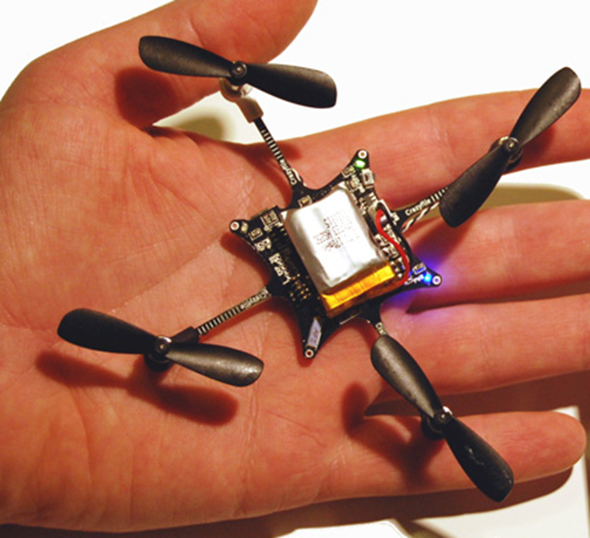
\includegraphics[scale = 0.25]{img/crazyflie.png}
      \caption{Crazyflie}
      \label{crazyflie}
    \end{figure}
    
    \section{Composants}
      L'objectif de cette section est de présenter les différents composants 
que nous avons utilisés pour construire ce premier drone.
      
      \subsection{Micro-contrôleur}
	Un micro-contrôleur est un \textit{system on chip}, c'est-à-dire une 
petite carte électronique proposant un certain nombre de fonctionnalités et 
pouvant fonctionner seule. C'est souvent un micro-processeur monté sur une 
carte avec plusieurs broches sur lesquelles l'utilisateur peut y connecter 
d'autres composants. Ainsi, il peut réaliser un montage complexe qu'il pourra 
utiliser en programmant le micro-processeur.
	Au début de notre année scolaire, nous avons eu un séminaire de cours 
pour nous apprendre le langage \textit{Arduino}. Nous avons pu découvrir un 
langage vraiment simple à prendre en main lorsque l'on a déjà quelques bases en 
programmation avec des langages comme le \textit{C}, ou le \textit{C++}. Nous 
nous sommes donc tournés vers les technologies proposées par Arduino pour le 
choix du micro-contrôleur. Finalement, nous avons opté pour une \textit{Arduino 
Pro Mini}. Le principal intérêt de cette carte se trouve dans sa petite taille 
et sa légèreté, 18 sur 33 millimètres pour seulement deux grammes. De plus elle 
propose un nombre suffisant de broches pour l'ensemble de notre montage.
	
	\begin{figure}
	  \begin{subfigure}{.5\textwidth}
	    \centering
	    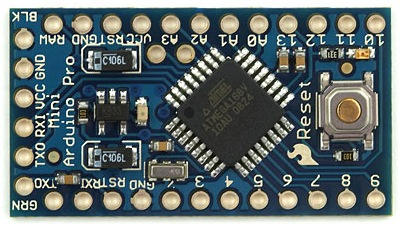
\includegraphics[scale=0.2]{img/arduinopromini.jpg}
	    \caption{Image de l'Arduino Pro Mini}
	    \label{imagearduino}
	  \end{subfigure}%
	  \begin{subfigure}{.5\textwidth}
	    \centering
	    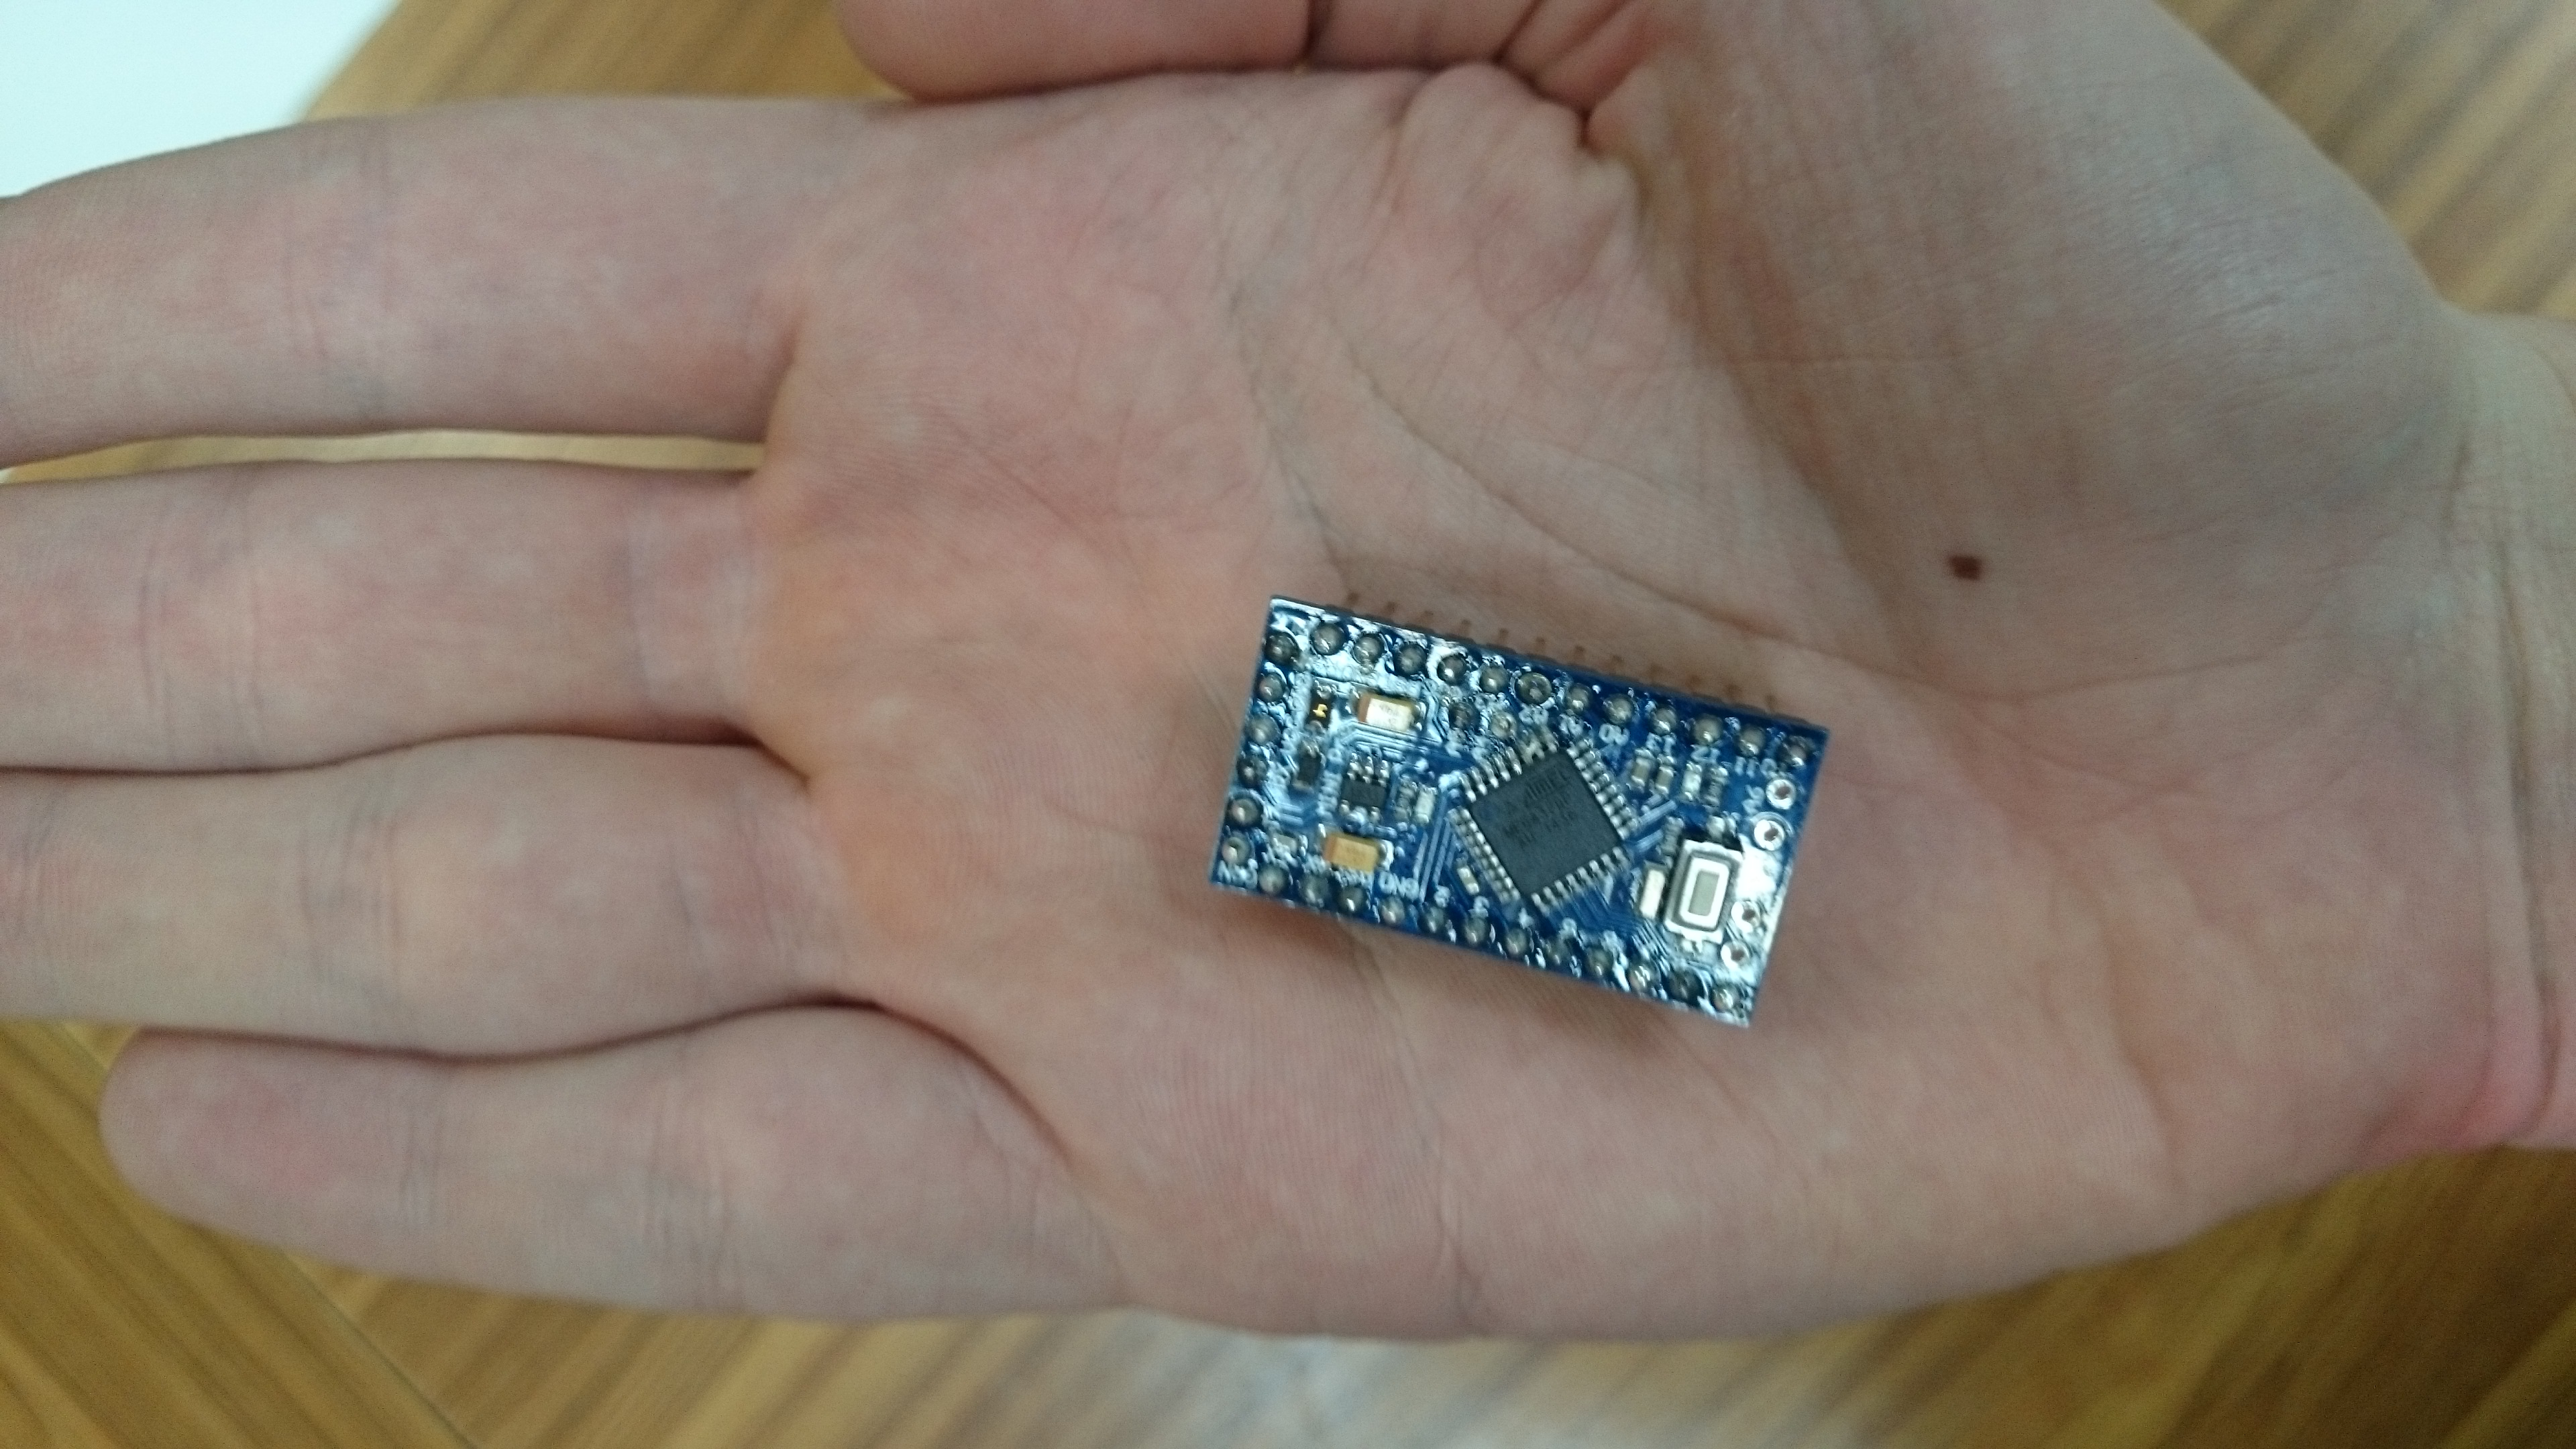
\includegraphics[scale=0.06]{img/arduino.JPG}
	    \caption{Photographie de notre Arduino Pro Mini}
	    \label{photoarduino}
	  \end{subfigure}
	  \caption{Image et photographie de l'Arduino Pro Mini}
	  \label{arduino}
	\end{figure}
	
      Une fois le micro-contrôleur en main, il nous faut ajouter d'autres 
composants nécessaires à la mise en place d'un drone. En branchant ces 
composants dans les trous sur l'extérieur de la carte nous pourrons les 
contrôler de manière logicielle, en codant le micro-processeur grâce au langage 
Arduino. Le micro-processeur, lui, se chargera de les faire fonctionner 
physiquement.  
	
      \subsection{Équilibrage et localisation}
	Il est important de disposer d'une technologie pour assister le drone à 
se stabiliser. Pour cela, ce dernier doit connaître "en permanence" son angle 
d'inclinaison. Nous avons donc besoin d'un gyroscope. Le large catalogue de 
modules Arduino propose une pièce qui fournit un gyroscope et un 
accéléromètre, le \textit{MPU-6050} (voir Figure \ref{mpu6050}). Ce module a 
une taille et un poids similaires à ceux du micro-contrôleur, 25.5 sur 15.2 
millimètres pour 1.5 grammes. Un autre point fort de ce circuit est qu'il est 
très utilisé au sein de la communauté Arduino. Il est donc facile de trouver 
des exemples d'utilisation.
	
	Pendant un certain moment nous nous sommes demandé comment nous 
pourrions connaître la position de notre drone dans l'espace. Naturellement 
nous avons pensé au GPS, mais la précision de ces technologies (pour rester 
dans 
un budget abordable) n'est clairement pas assez précise. Bien entendu, dans le 
cadre où le drone devrait faire son analyse en extérieur sur une zone assez 
grande, les GPS sont intéressants. Mais notre drone devra simplement analyser 
une salle de classe, alors une précision "au mètre près" est beaucoup trop 
large. Nous aurions plutôt besoin d'une précision de l’ordre du décimètre.  Une 
autre solution a été évoquée, créer notre propre système de localisation, en 
créant une triangulation\cite{triangulation} à l’aide d’un réseau d’antennes. 
Ce principe consiste à placer trois antennes autour d'une zone et qui emmettent 
un signal.
L'objet que l'on souhaite localiser réceptionne ces signaux. Il détermine alors 
la distance qui le sépare des émetteurs. À l'aide de ces trois distances, on 
est alors en mesure de déterminer sa position dans l'espace. Toutefois, pour 
des raisons de coûts, cette solution ne nous semble pas viable sur notre drone. 
Aussi, elle n'est pas conforme à la problématique de notre projet, puisque nous 
partons du principe que nous ne connaissons pas l'étendue de la zone. Ainsi, 
nous ne serions pas en mesure de placer nos antennes en périphérie de la zone.

	Finalement une connaissance, nous a conseillé de travailler avec un 
accéléromètre. Un accéléromètre est un module permettant de mesurer 
l'accélération linéaire d’un système. En connaissant l'accélération de notre 
drone, il sera alors possible de déterminer sa vitesse et donc, ses 
déplacements 
dans l’espace. Nous avons donc choisi de nous tourner vers cette solution. 
C'est aussi pour cette raison que nous avons choisi le MPU-6050 car il embarque 
un accéléromètre.
	
	    \begin{figure}
	      \begin{subfigure}{.5\textwidth}
		\centering
		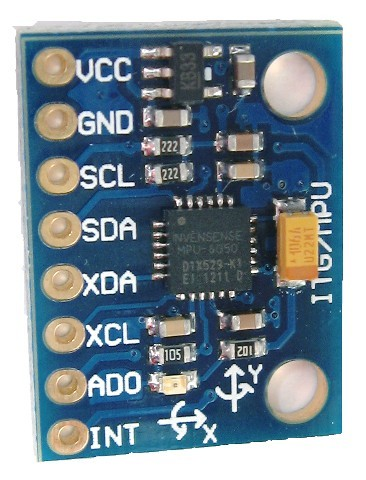
\includegraphics[scale=0.2]{img/mpu-6050.jpg}
		\caption{Image du MPU-6050}
		\label{imagempu6050}
	      \end{subfigure}%
	      \begin{subfigure}{.5\textwidth}
		\centering
		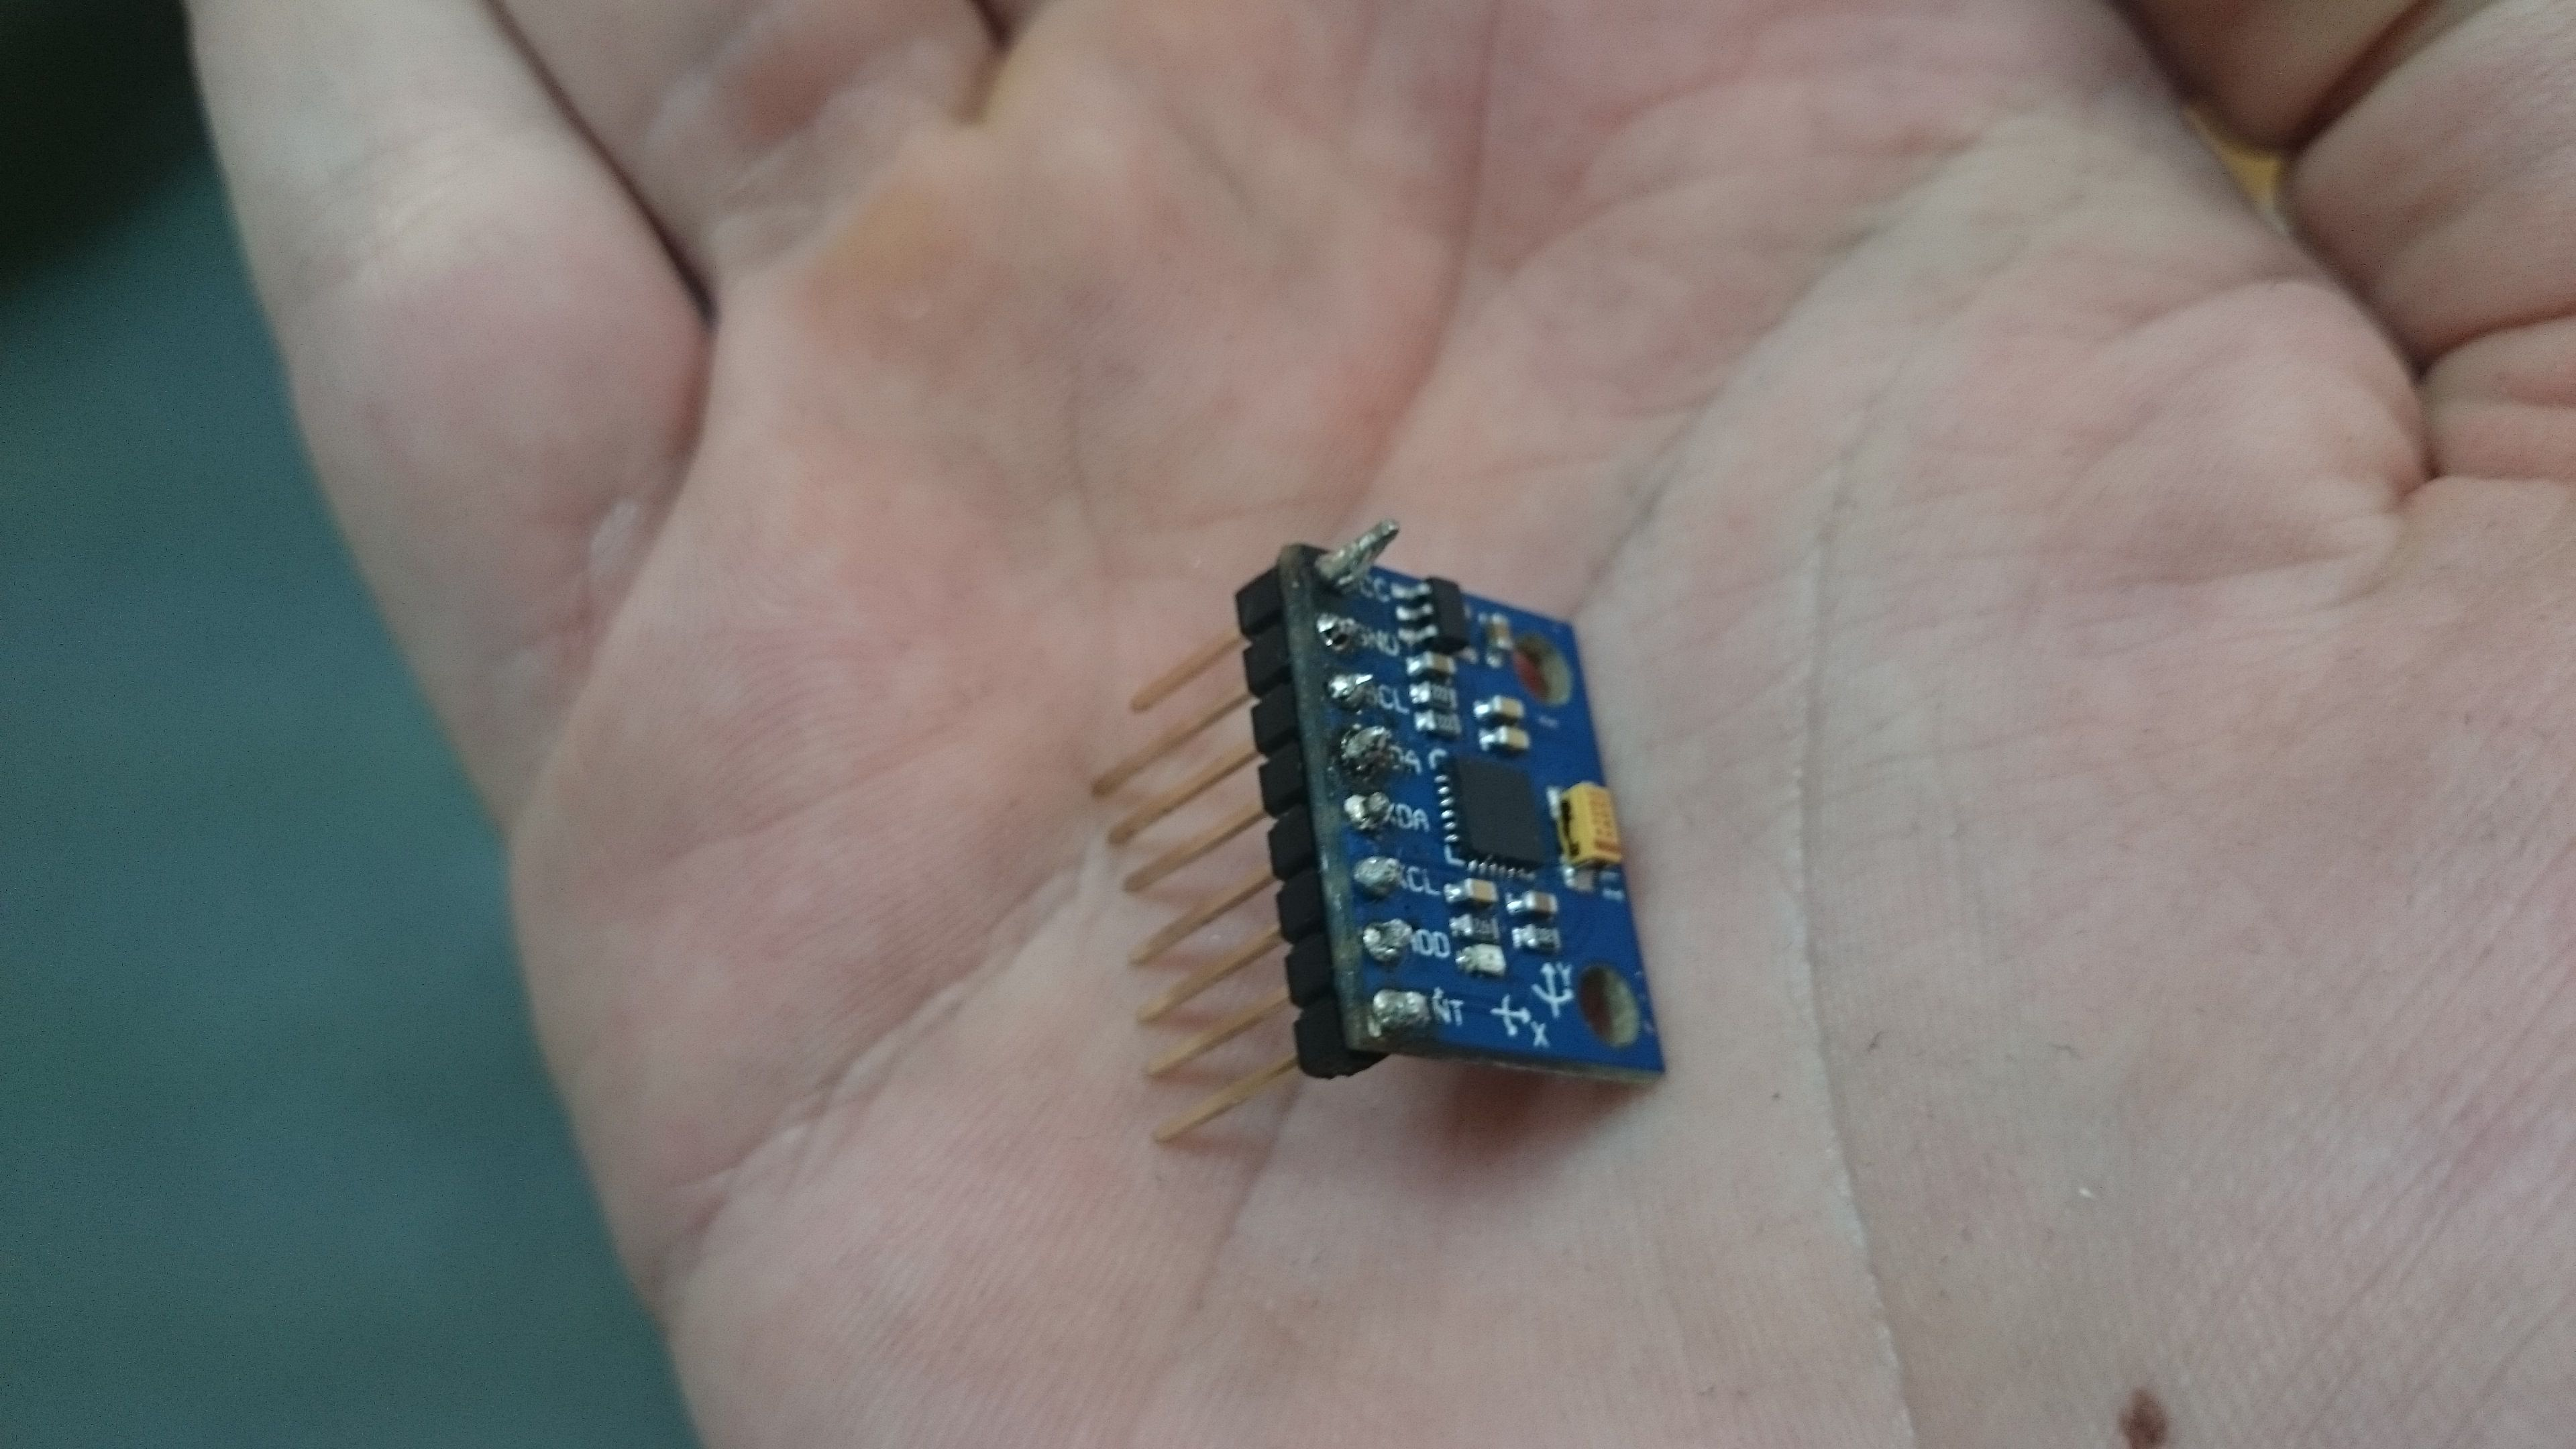
\includegraphics[scale=0.06]{img/mpu6050.jpg}
		\caption{Photographie de notre MPU-6050}
		\label{photompu6050}
	      \end{subfigure}
	      \caption{Image et photographie du MPU-6050}
	      \label{mpu6050}
	    \end{figure}
	    
	Pour pouvoir utiliser ce composant nous avons utilisé la bibliothèque 
développée par Jeff Rowberg\cite{jeff_rowberg_lib}. Ses travaux permettent de 
représenter logiciellement un gyroscope et de récupérer les valeurs calculées 
par le MPU-6050. Ainsi, en récupérant ces mesures nous pouvons déterminer la 
puissance requise pour chaque moteur afin d'équilibrer le drone.

	Vous pouvez retrouver nos recherches à propos du fonctionnement d'un 
gyroscope, dans l'Annexe B de ce rapport.

	En cours de développement nous nous sommes rendu compte que déterminer 
la position du drone dans l'espace avec seulement un accéléromètre n'est pas 
une solution envisageable. En effet, afin de calculer cette position il faut 
intégrer deux fois les mesures renvoyées par le capteur. Or, à chaque 
intégration s'introduit une petite erreur. Mais la double intégration fait que 
nos calculs suivent une erreur quadratique. Ainsi, il nous serait peut-être 
possible de déterminer correctement une première position, mais au fil de 
l'exécution de l'application, nos calculs seraient complètement faussés. Il 
faut savoir que la problématique de déterminer la position dans l'espace d'un 
objet en mouvement dans un endroit fermé est encore au stade de la recherche. 
Cette problématique pourrait faire un sujet de projet de fin d'études à elle 
toute seule.
      
      \subsection{Communication avec le serveur}
	Afin que le drone puisse communiquer avec le serveur nous avons dans un 
premier temps pensé à utiliser des modules \textit{XBee}, qui utilisent le 
protocole de communication sans fil, défini par le standard \textit{IEEE 
802.15.4} et qui sont très répendus au sein de la communauté Arduino. De plus 
il semblerait que ces composants soient très simples d'utilisation et que la 
qualité des signaux soit très fiable. Toutefois, les modules \textit{XBee} 
sont relativement chers (23 \euro) dû au fait que le protocole utilisé soit 
breveté, nous nous sommes alors penchés vers une autre technologie. Nous avons 
finalement opté pour un module de transmission/réception radio à fréquence 
2.4GHz (voir Figure \ref{nrf24l01}). Ils sont eux aussi très répendus chez les 
utilisateurs d'Arduino. Comme pour les autres composants que nous avons 
choisis, il est bon marché (0.8 \euro) et d'une taille de 15 sur 29 millimètres 
pour deux grammes.
	
	    \begin{figure}
	      \begin{subfigure}{.5\textwidth}
		\centering
		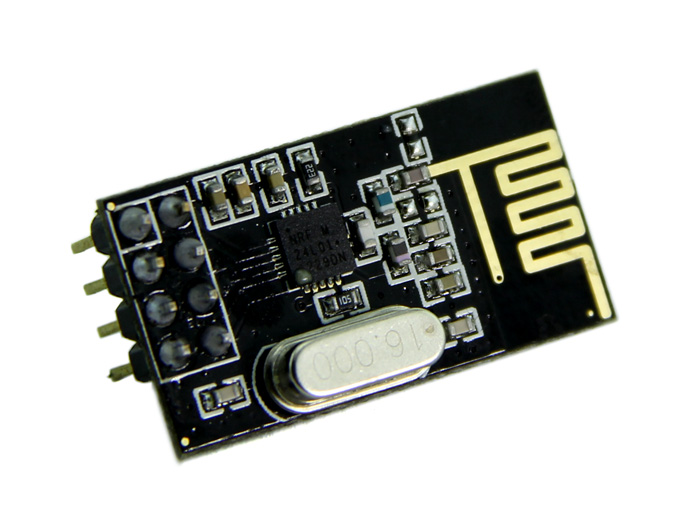
\includegraphics[scale=0.4]{img/image_nrf24l01.jpg}
		\caption{Image du NRF24L01}
		\label{imagenrf24L01}
	      \end{subfigure}%
	      \begin{subfigure}{.5\textwidth}
		\centering
		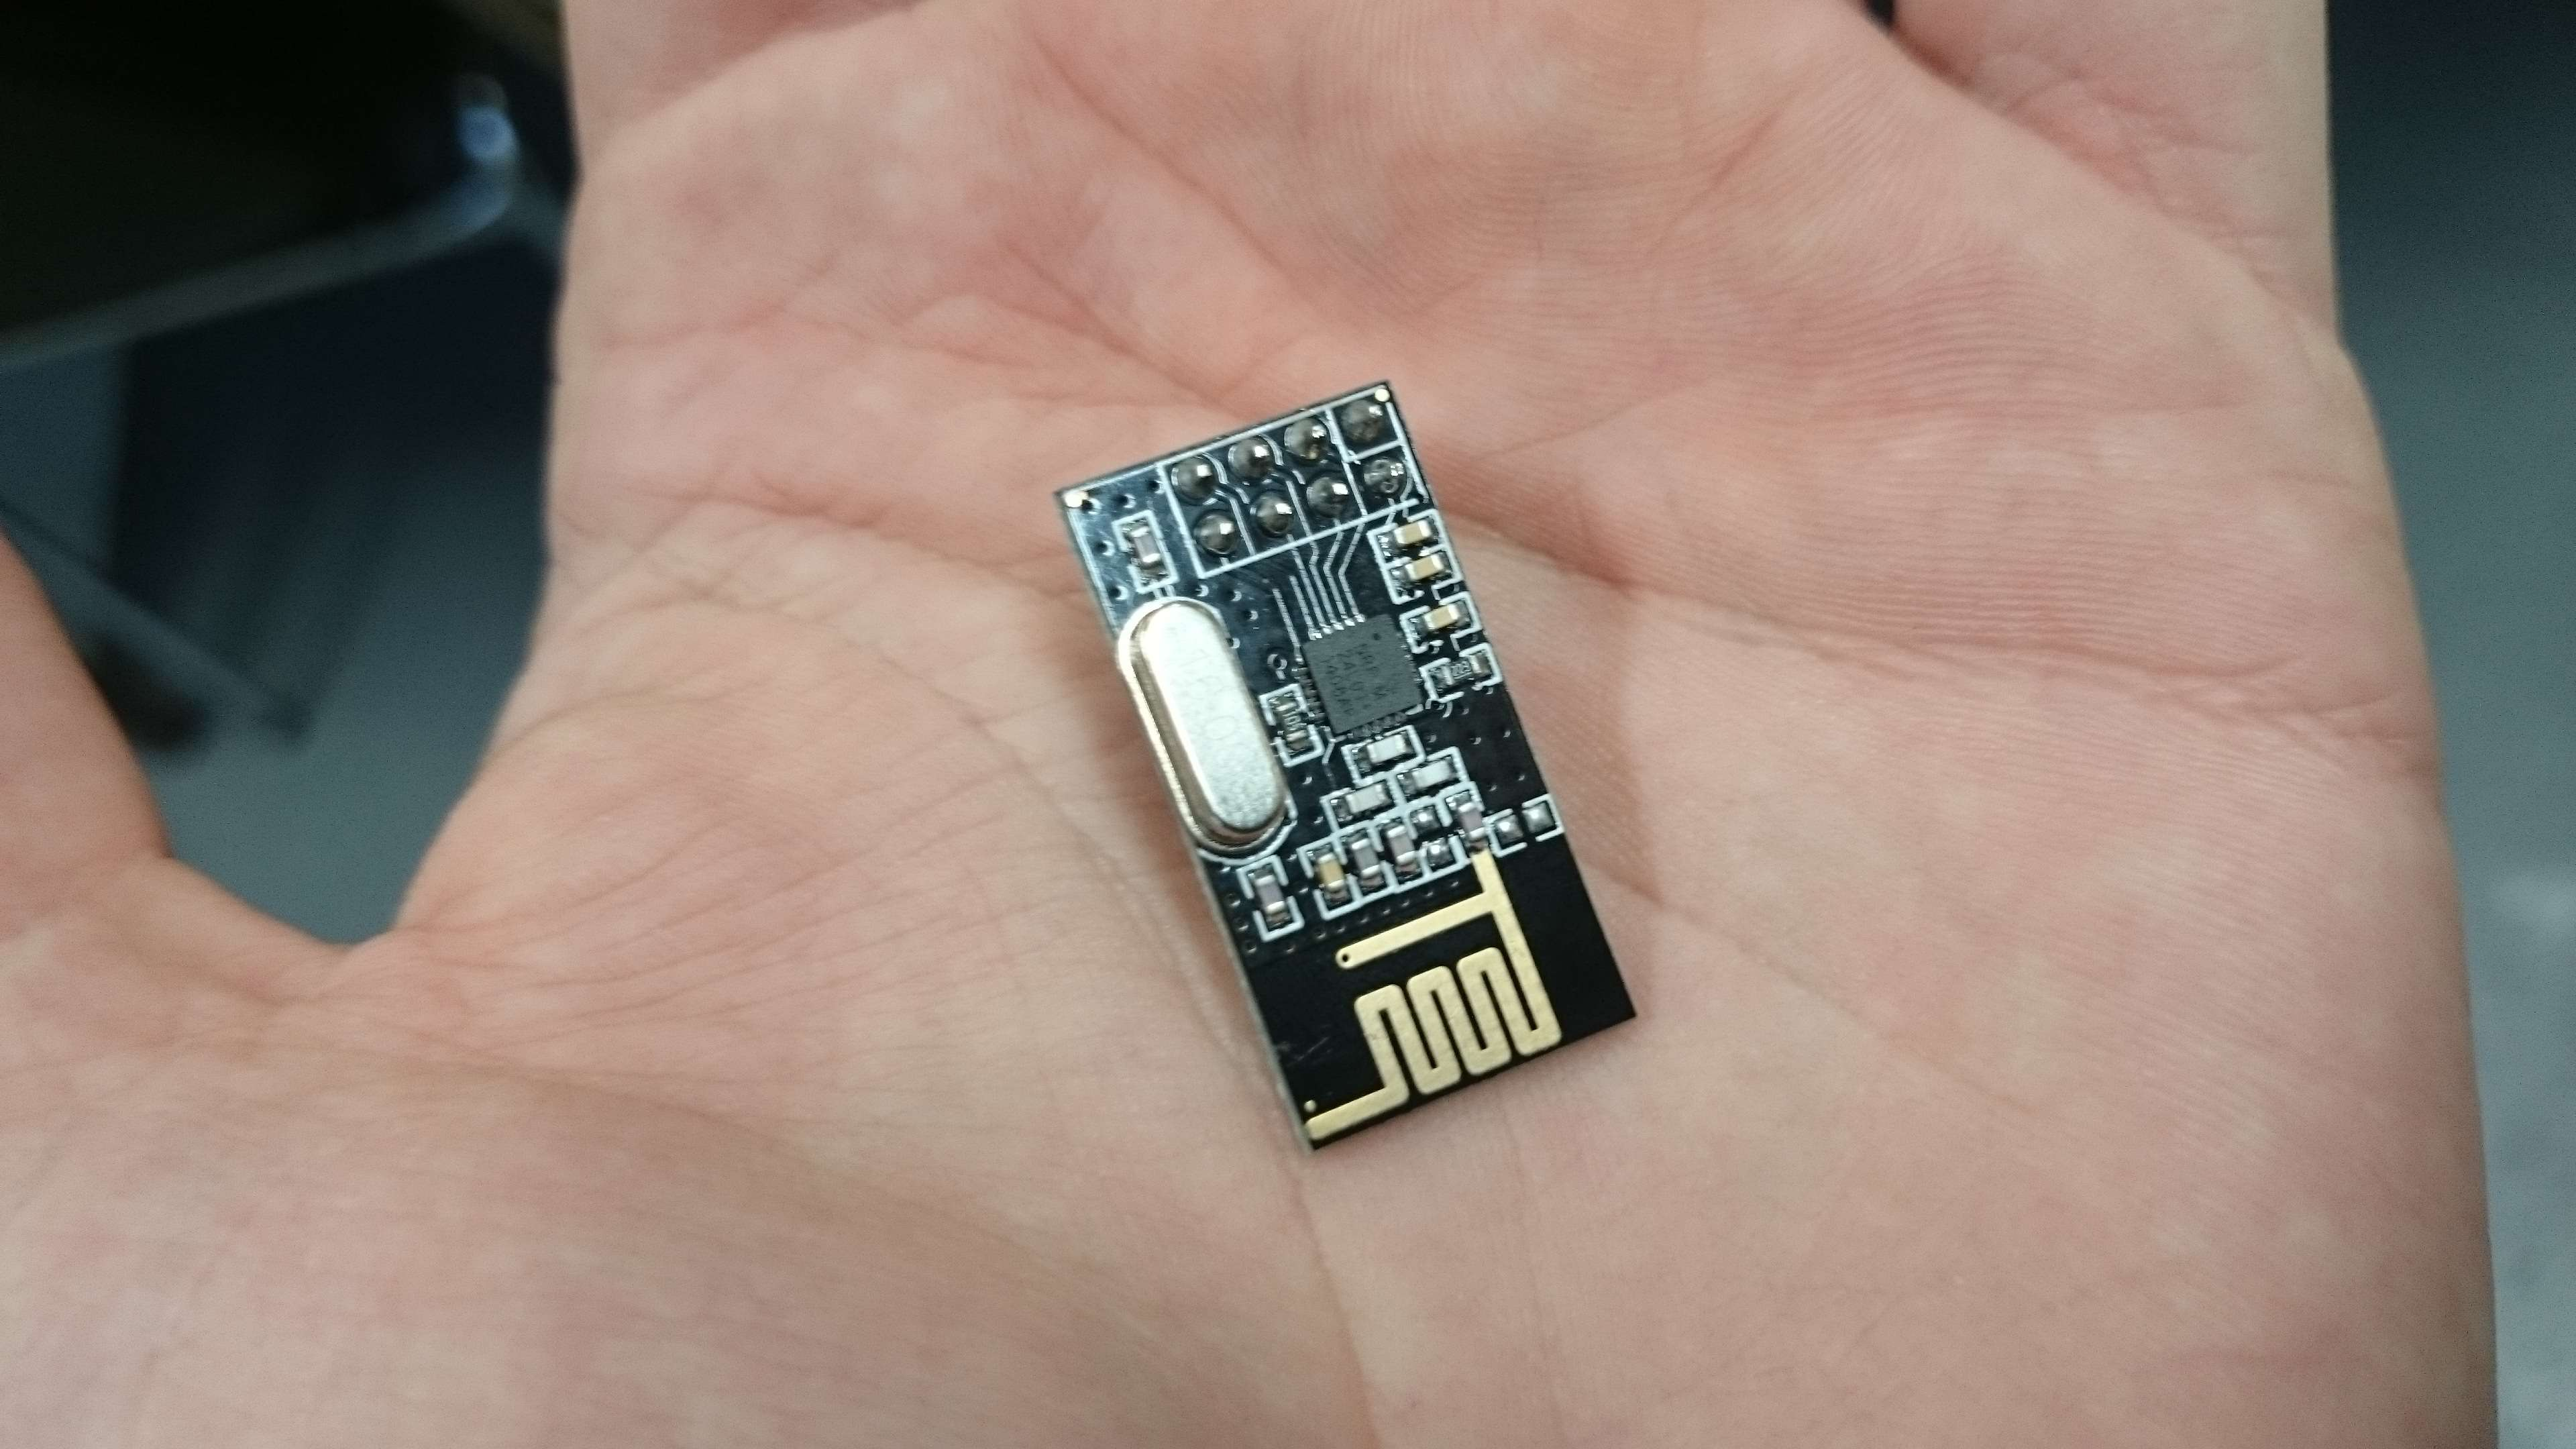
\includegraphics[scale=0.06]{img/nrf24l01.jpg}
		\caption{Photographie de notre NRF24L01}
		\label{photonrf24L01}
	      \end{subfigure}
	      \caption{Image et photographie du NRF24L01}
	      \label{nrf24l01}
	    \end{figure}
	    
	Cependant ces composants sont un peu plus compliqués à prendre en main. 
Mais heureusement, il existe de nombreuses bibliothèques. Nous avons donc créé 
une surcouche de la bibliothèque \textit{RadioHead}\cite{radiohead}. Cette 
bibliothèque permet de représenter logiciellement un transmetteur radio. À 
partir de cet objet il est possible d'envoyer et lire des messages en 
fournissant une adresse (qui représente un port entre le transmetteur et le 
récepteur qui est une autre instance de ce composant, sur une autre plaquette 
Arduino). Notre surcouche nous permet de vérifier le bon envoi et la bonne 
réception des données en retournant un code d'erreur en cas d'échec.

	Toute fois le très faible coût de ces composants se ressent directement 
sur la fiabilité de leur signauxs. En effet, l'envoi et la réception des 
données est malheureusement un peu aléatoire. Il n'est pas rare de ne recevoir 
qu'un message sur deux.
	
      
      \subsection{Contrôle moteur}
	La plupart des drones embarquent un \textit{Electronic Speed Controler} 
(\textit{ESC}) pour chaque moteur. Ces composants servent à contrôler la 
vitesse du moteur ainsi que son sens de rotation. Il faut savoir qu'un ESC vaut 
environ 16 \euro. Ce qui fait 64 \euro \space pour un quadcopter. Outre le prix 
important de ces modules, leur poids (25 grammes/module) aussi nous oblige à 
nous orienter vers une autre solution. Nous avons donc pensé à créer nos 
propres 
ESC simplement en branchant un transistor entre chaque moteur et les broches de 
sortie de l’Arduino. Les transistor ont pour propriété de fonctionner comme des 
interrupteurs électriques. Ainsi en couplant les variations du signal 
électrique généré par l'Arduino et la propriété du transistor nous obtenons un 
ESC fait main.

      \subsection{Moteurs}
	Dans l'introduction nous avons expliqué que nous utilisons les mêmes 
moteurs que ceux du Crazyflie. Cependant, comme pour les autres composants il 
faut coder en Arduino leur contrôle. Ainsi nous avons implémenté une petite 
bibliothèque permettant de représenter logiciellement parlant, un moteur. Cet 
objet possède alors une méthode permettant de modifier sa vitesse. Vitesse qui 
sera alors modifiée logiciellement puis physiquement.

      \subsection{Mesure de la topographie}
	Pour mesurer une distance il existe plusieurs types de capteurs 
différents, comme par exemple un laser. Cependant, nous ne possédons pas ce 
genre d'outil mais lors du séminaire d'Arduino du début d'année nous avons 
utilisé des capteurs ultrasons (\textit{HC-SR04}). Pour ce projet nous avons 
donc choisi de réutiliser ces capteurs (pour des raisons économiques). 
Toutefois, dû aux propriétés du déplacement d'une onde sonore dans l'espace, ce 
genre de capteur n'est pas ce qu'il y a de plus fiable. L'onde sonore se 
répendant sous une forme d'arc de cercle, on ne peut pas savoir avec certitude 
quel point précisément à été mesuré.

	\begin{figure}[htbp]%Photo de l'Arduino
	  \centering
	  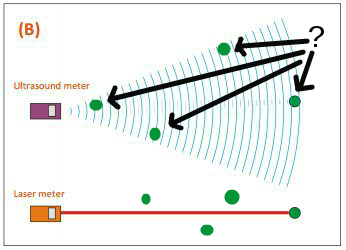
\includegraphics[scale = 0.5]{img/sonarwave.png}
	  \caption{Comparaison des fiabilités de mesure}
	  \label{sonarwave}
	\end{figure}
	
	Mais dans le cadre de la présentation de notre application ce problème 
ne sera pas vraiment dérengeant.
	
	\begin{figure}
	  \begin{subfigure}{.5\textwidth}
	    \centering
	    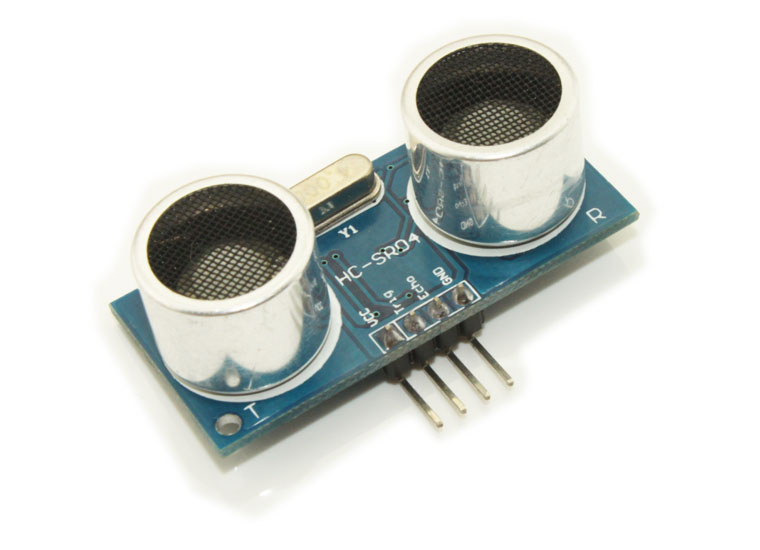
\includegraphics[scale=0.2]{img/image_hcsr04.jpg}
	    \caption{Image du HC-SR04}
	    \label{imagehcsr04}
	  \end{subfigure}%
	  \begin{subfigure}{.5\textwidth}
	    \centering
	    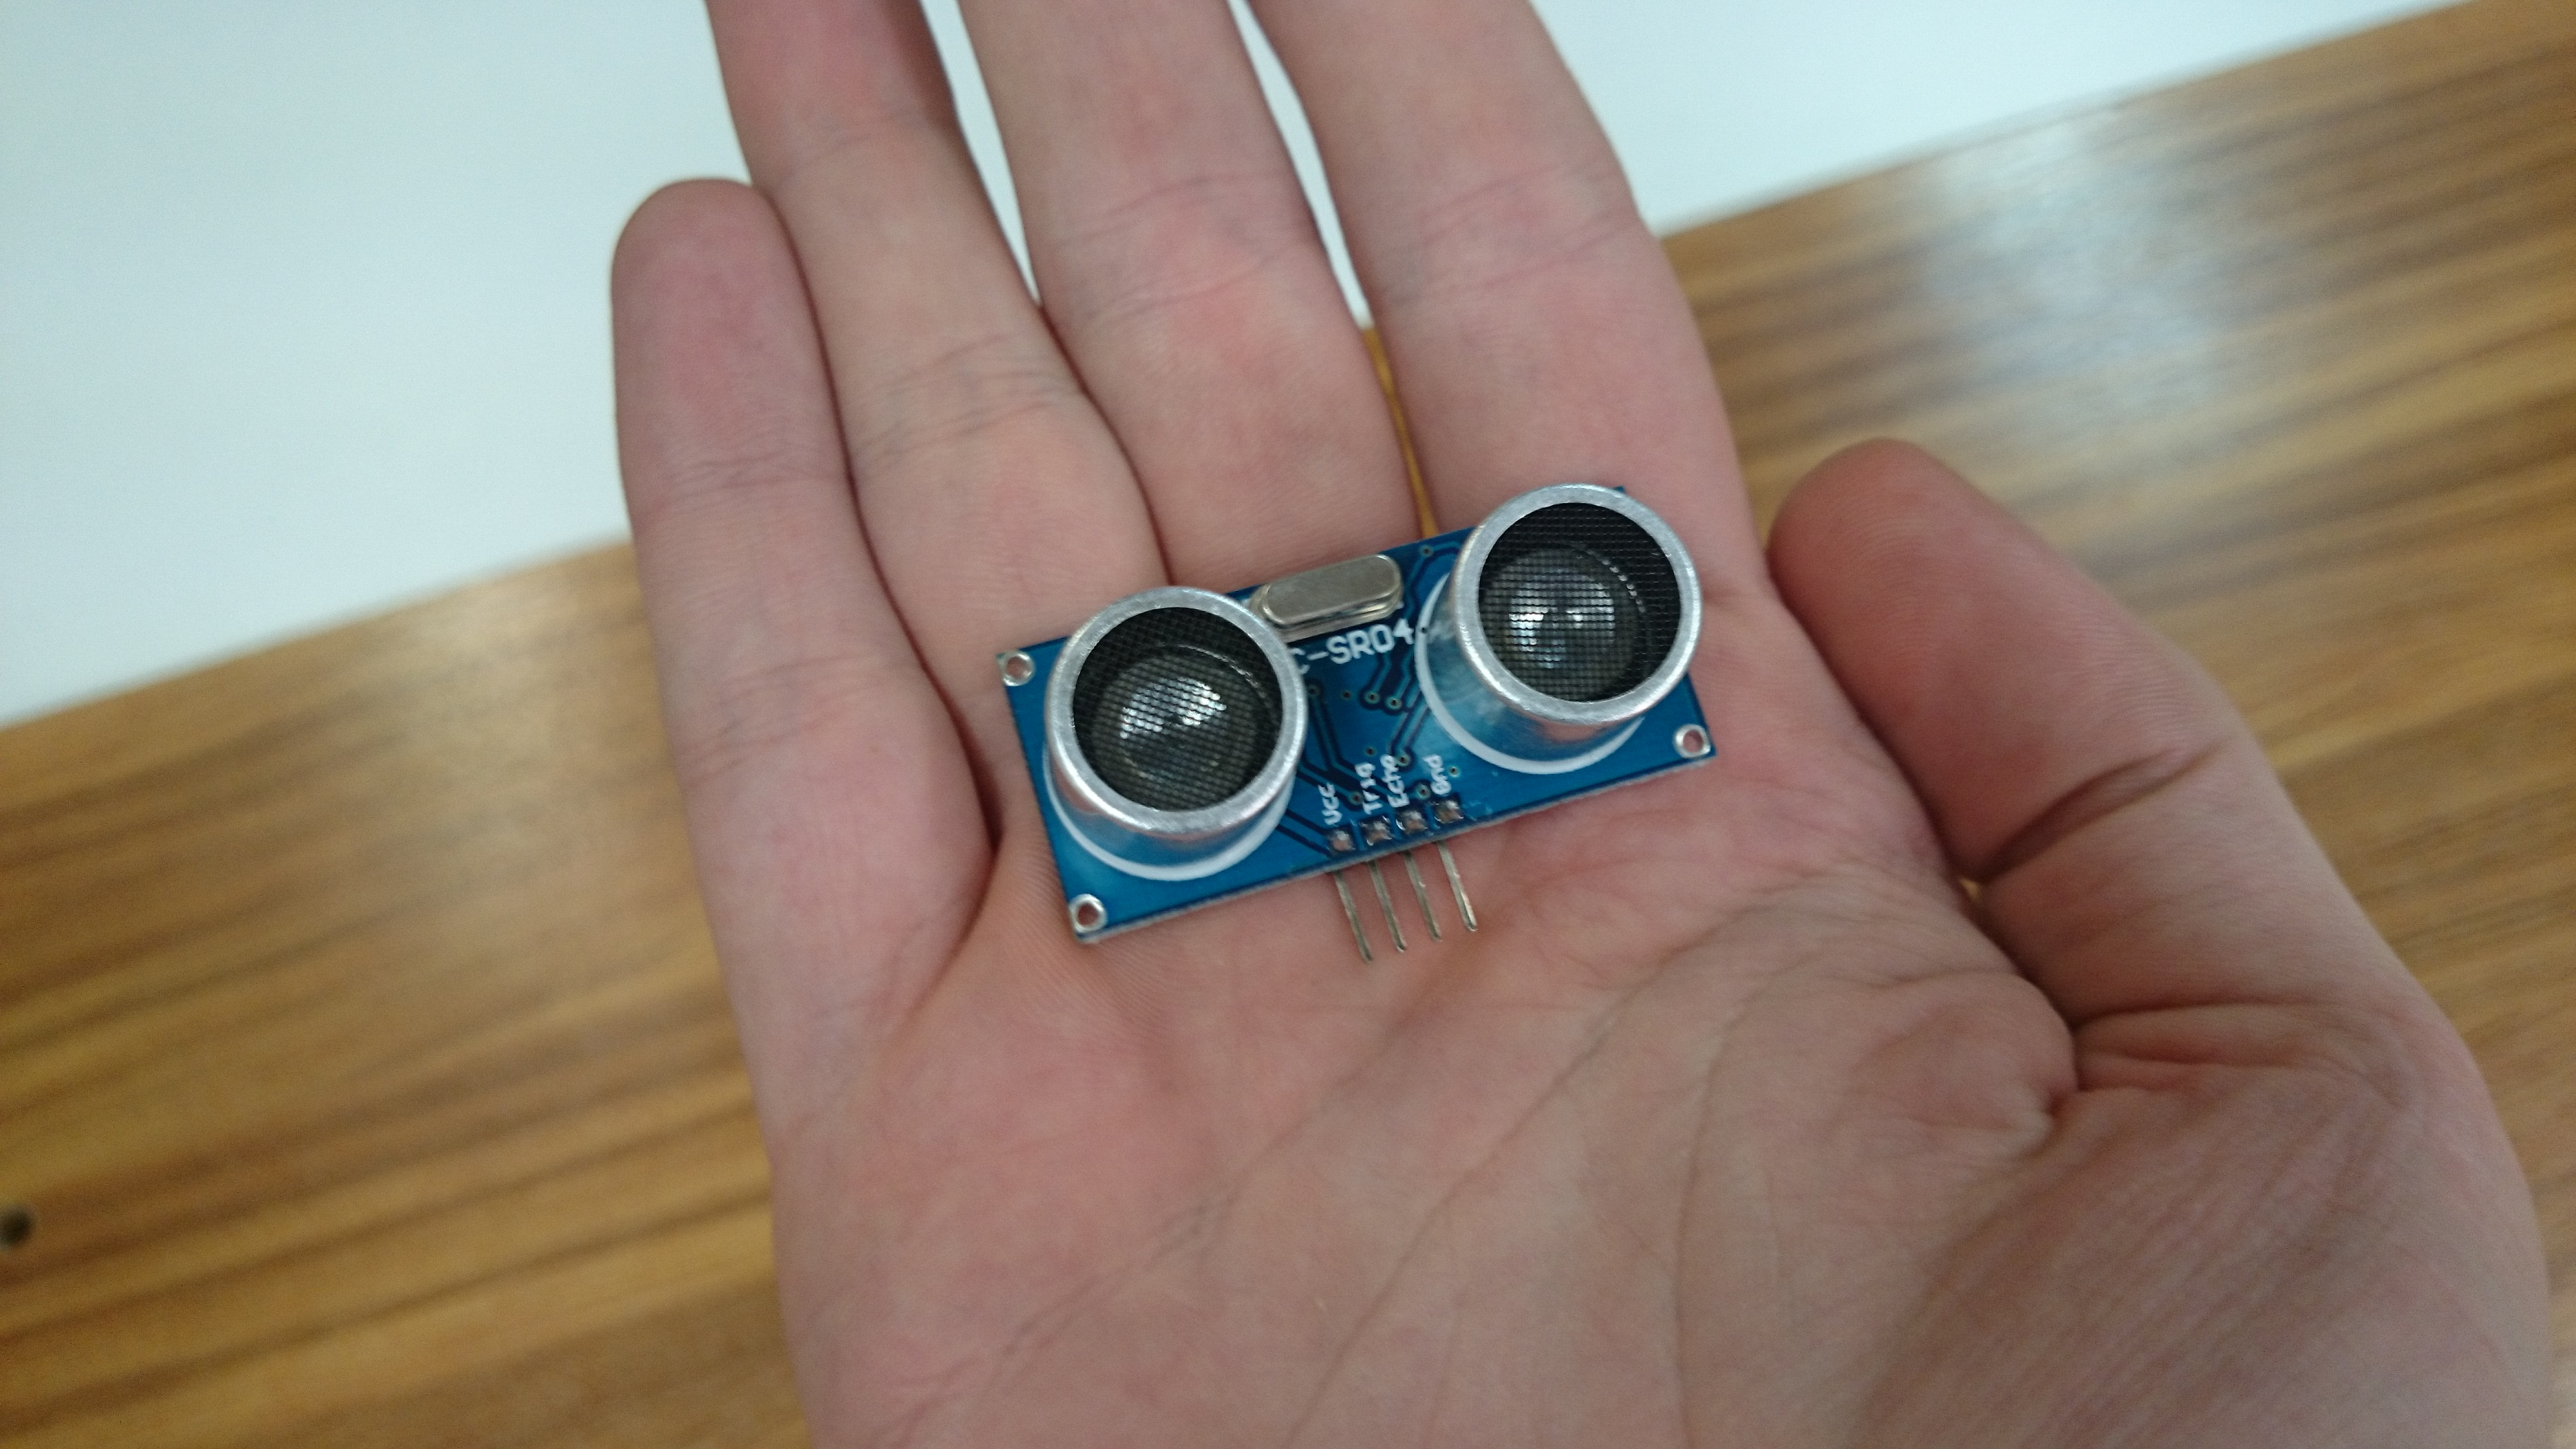
\includegraphics[scale=0.06]{img/hcsr04.JPG}
	    \caption{Photographie de notre HC-SR04}
	    \label{photohcsr04}
	  \end{subfigure}
	  \caption{Image et photographie du HC-SR04}
	  \label{hcsr04}
	\end{figure}
	
	Le HC-SR04 (voir Figure \ref{hcsr04}) est lui aussi un composant très 
répendu au sein de la communauté Arduino. Ainsi nous pouvons directement 
utiliser une bibliothèque déjà implémentée, \textit{NewPing}\cite{newping}. 
Elle permet de représentée logiciellement un capteur ultrasons et de calculer 
la distance d'un point par rapport au montage en mesurant le temps de retour de 
l'onde sonore.
	
    \section{Assemblage}
      Une fois tous les composants reçus et une fois toutes les bibliothèques 
développées nous avons pu assembler le tout. Toutefois, il restait encore deux 
pièces manquantes au puzzle. En effet, il manquait encore le circuit qui relit 
tous les composants à l'Arduino et un moyen de fixer les moteurs au drone. 
Cependant ces deux éléments ne sont pas des articles que l'on peut acheter sur 
un site de vente. Nous allons expliquer dans cette section comment nous avons 
obtenu ces deux dernières pièces et présenter le résultat après assemblage.

      \subsection{Circuit}
	Pour pouvoir assembler tous les composants ensemble il faut réaliser un 
circuit imprimé. Pour cela nous avons utilisé le logiciel 
\textit{Fritzing}\cite{fritzing}. C'est un logiciel libre qui permet de 
réaliser des schémas électroniques ainsi que le PCB associé (c'est à dire le 
dessin qui va servir à la production du circuit). Ce logiciel propose de base 
un large catalogue de composants mais il est aussi possible de créer les siens. 
De plus, un grand nombre de personnes utilisent ce logiciel, ce qui permet 
dans la plupart des cas de ne pas avoir à créer de composants puisqu'il y a de 
grandes chances que des utilisateurs les aient déjà dessinés.

      \begin{figure}[htbp]%PCB du premier drone
	\centering
	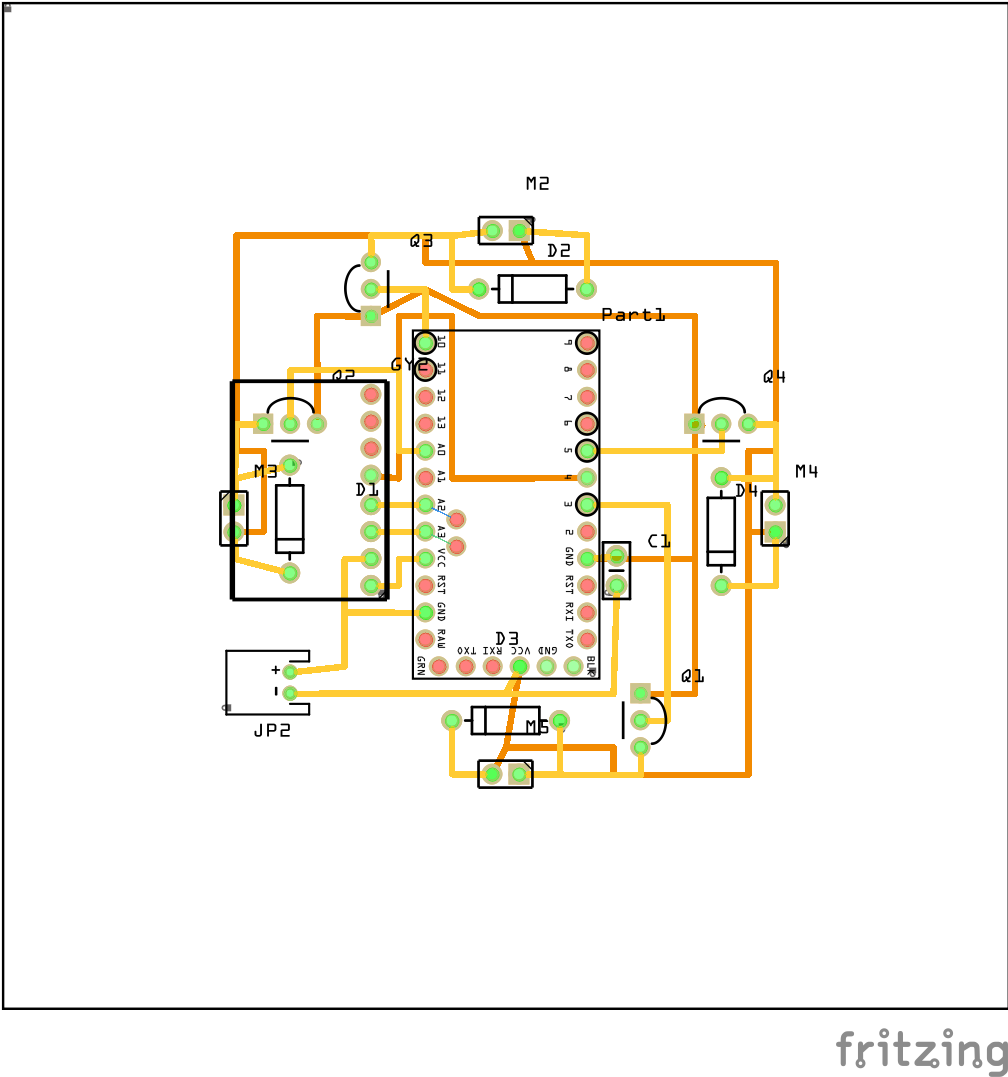
\includegraphics[scale = 0.9]{img/nouveau_drone_circuit_pcb.png}
	\caption{PCB du drone}
	\label{pcb1drone}
      \end{figure}
      
      La Figure \ref{pcb1drone} représente le PCB de notre drone. C'est le type 
de dessin qui servent à la production de circuits imprimés. Le dessin d'un PCB 
est une étape obligatoire dans la production d'un montage électronique car un 
circuit dépend du résultat attendu. Le montage entre un drone et un ordinateur 
ne sera pas le même et même le montage entre un drone et un autre modèle de 
drone sera différent. C'est pour cette raison qu'on ne peut pas acheter un 
circuit déjà fait.
      
      \subsection{Fixations moteur}
	Comme nous nous sommes inspirés du Crazyflie, nous avons fait le choix 
de ne pas utiliser de châssis. Ces composants sont assez compliqués à choisir, 
car il faut choisir entre un matériau léger mais coûteux et un matériau "lourd" 
et bon marché. Donc nous avons pensé que le circuit pourrait lui-même faire 
office de châssis. Bien entendu, ce choix est risqué car le drone est plus 
fragile. Mais notre application n'est pas vraiment "à risque" dans le sens où 
notre drone n'est pas censé faire des acrobaties et que nous comptions mettre 
en place des sécurités pour qu'il évite les obstacles de son environnement.

	De plus les moteurs du Crazyflie ont une dimension assez particulière. 
Habituellement les moteurs de drone sont plus gros donc il serait difficile de 
trouver un châssis qui soit compatible avec nos moteurs. De plus, souvent les 
moteurs de drone se vissent sur le châssis, mais les moteurs du Crazyflie ne 
possèdent pas de pas de vis. Nous étions donc dépendant de la solution utilisé 
par le Crazyflie, c'est à dire utiliser des petites pièces en plastique qui se 
chargent de fixer les moteurs au circuit imprimé.

	Ces fixations ne sont pas disponibles à la vente. Cependant, BitCraze a 
déposé le fichier de modélisation sur leur compte GitHub\cite{gitbit}. Ainsi, 
nous avons pu télécharger ce fichier afin de le fournir à une imprimante 3D 
pour produire les pièces qu'il nous fallait.

      \begin{figure}[htbp]%PCB du premier drone
	\centering
	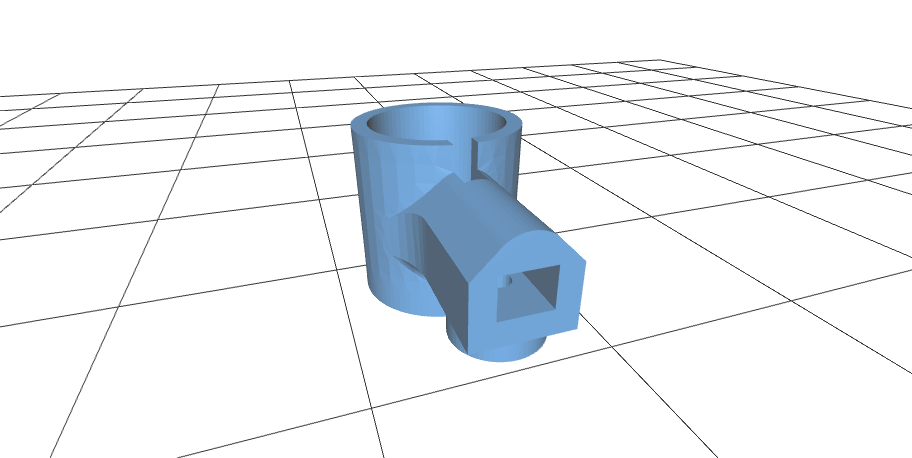
\includegraphics[scale = 0.4]{img/model_fixation.png}
	\caption{Modèle de fixation moteur}
	\label{fixationmodel}
      \end{figure}
      
	La Figure \ref{fixationmodel} est une capture d'écran du fichier de 
modélisation des fixations moteurs.

      \subsection{Production des pièces manquantes}
	L'EISTI étant une école d'ingénieur informatique, elle ne dispose ni 
du matériel nécessaire pour la production de circuit imprimé, ni d'imprimante 
3D pour imprimer nos fixations moteur. Ainsi, nous avons dû chercher une entité 
externe à notre école pour pouvoir obtenir nos deux dernières pièces. 

	Dans un premier temps nous avons pensé à nous servir du 
fablab\cite{faclab} de l'université de Cergy-Pontoise. Cet atelier se trouve à 
Gennevilliers (92), il propose un grand nombre d'outils mis à disposition 
gratuitement. La seule contrepartie est de donner de son temps à la vie du 
laboratoire. Toutefois pour utiliser certaines machines comme les imprimantes 
3D (de qualité), les découpeuses lazer, les fraiseuses, etc... il est 
nécessaire de suivre une formation. Les gérants étant conscients que nous 
sommes soumis à des deadlines, nous ont proposé de faire les choses à notre 
place. En échange nous devions simplement faire des formations sur 
l'utilisation du logiciel Fritzing et sur la fabrication d'un drone. Ils nous 
ont alors demandé de leur envoyer un mail afin qu'on puisse rester en contact. 
Ce que nous avons fait au retour de notre visite. Cependant, nous n'avons 
jamais obtenu de réponse.

      Nous avons alors cherché un autre moyen. Il existe des entreprises qui 
disposent de quelques imprimantes 3D. Elles les mettent alors à disposition du 
public contre une petite somme d'argent. Nous avons envoyé une commande, à 
l'aide du fichier de modélisation. Mais notre demande s'est vue être refusée 
car leurs imprimantes ne sont pas assez précises pour nos besoins.

      À cette même époque, notre école accueillait le concours annuel de 
robotique, \textit{RobAFIS}\cite{robafis}. Durant la compétition des 
entreprises exposaient leurs produits. Notamment \textit{Polytech 
Instrumentation}\cite{polytechinstru} (une filiale de 
\textit{Jeulin}\cite{jeulin}) exposait des imprimantes 3D. Nous en avons alors 
profité pour leur demander s'ils accepteraient de nous imprimer nos pièces. Ils 
ont alors accepté et nous avons reçu nos pièces (voir Figure \ref{fixation}) 
par courrier deux semaines plus tard.

      \begin{figure}[htbp]%PCB du premier drone
	\centering
	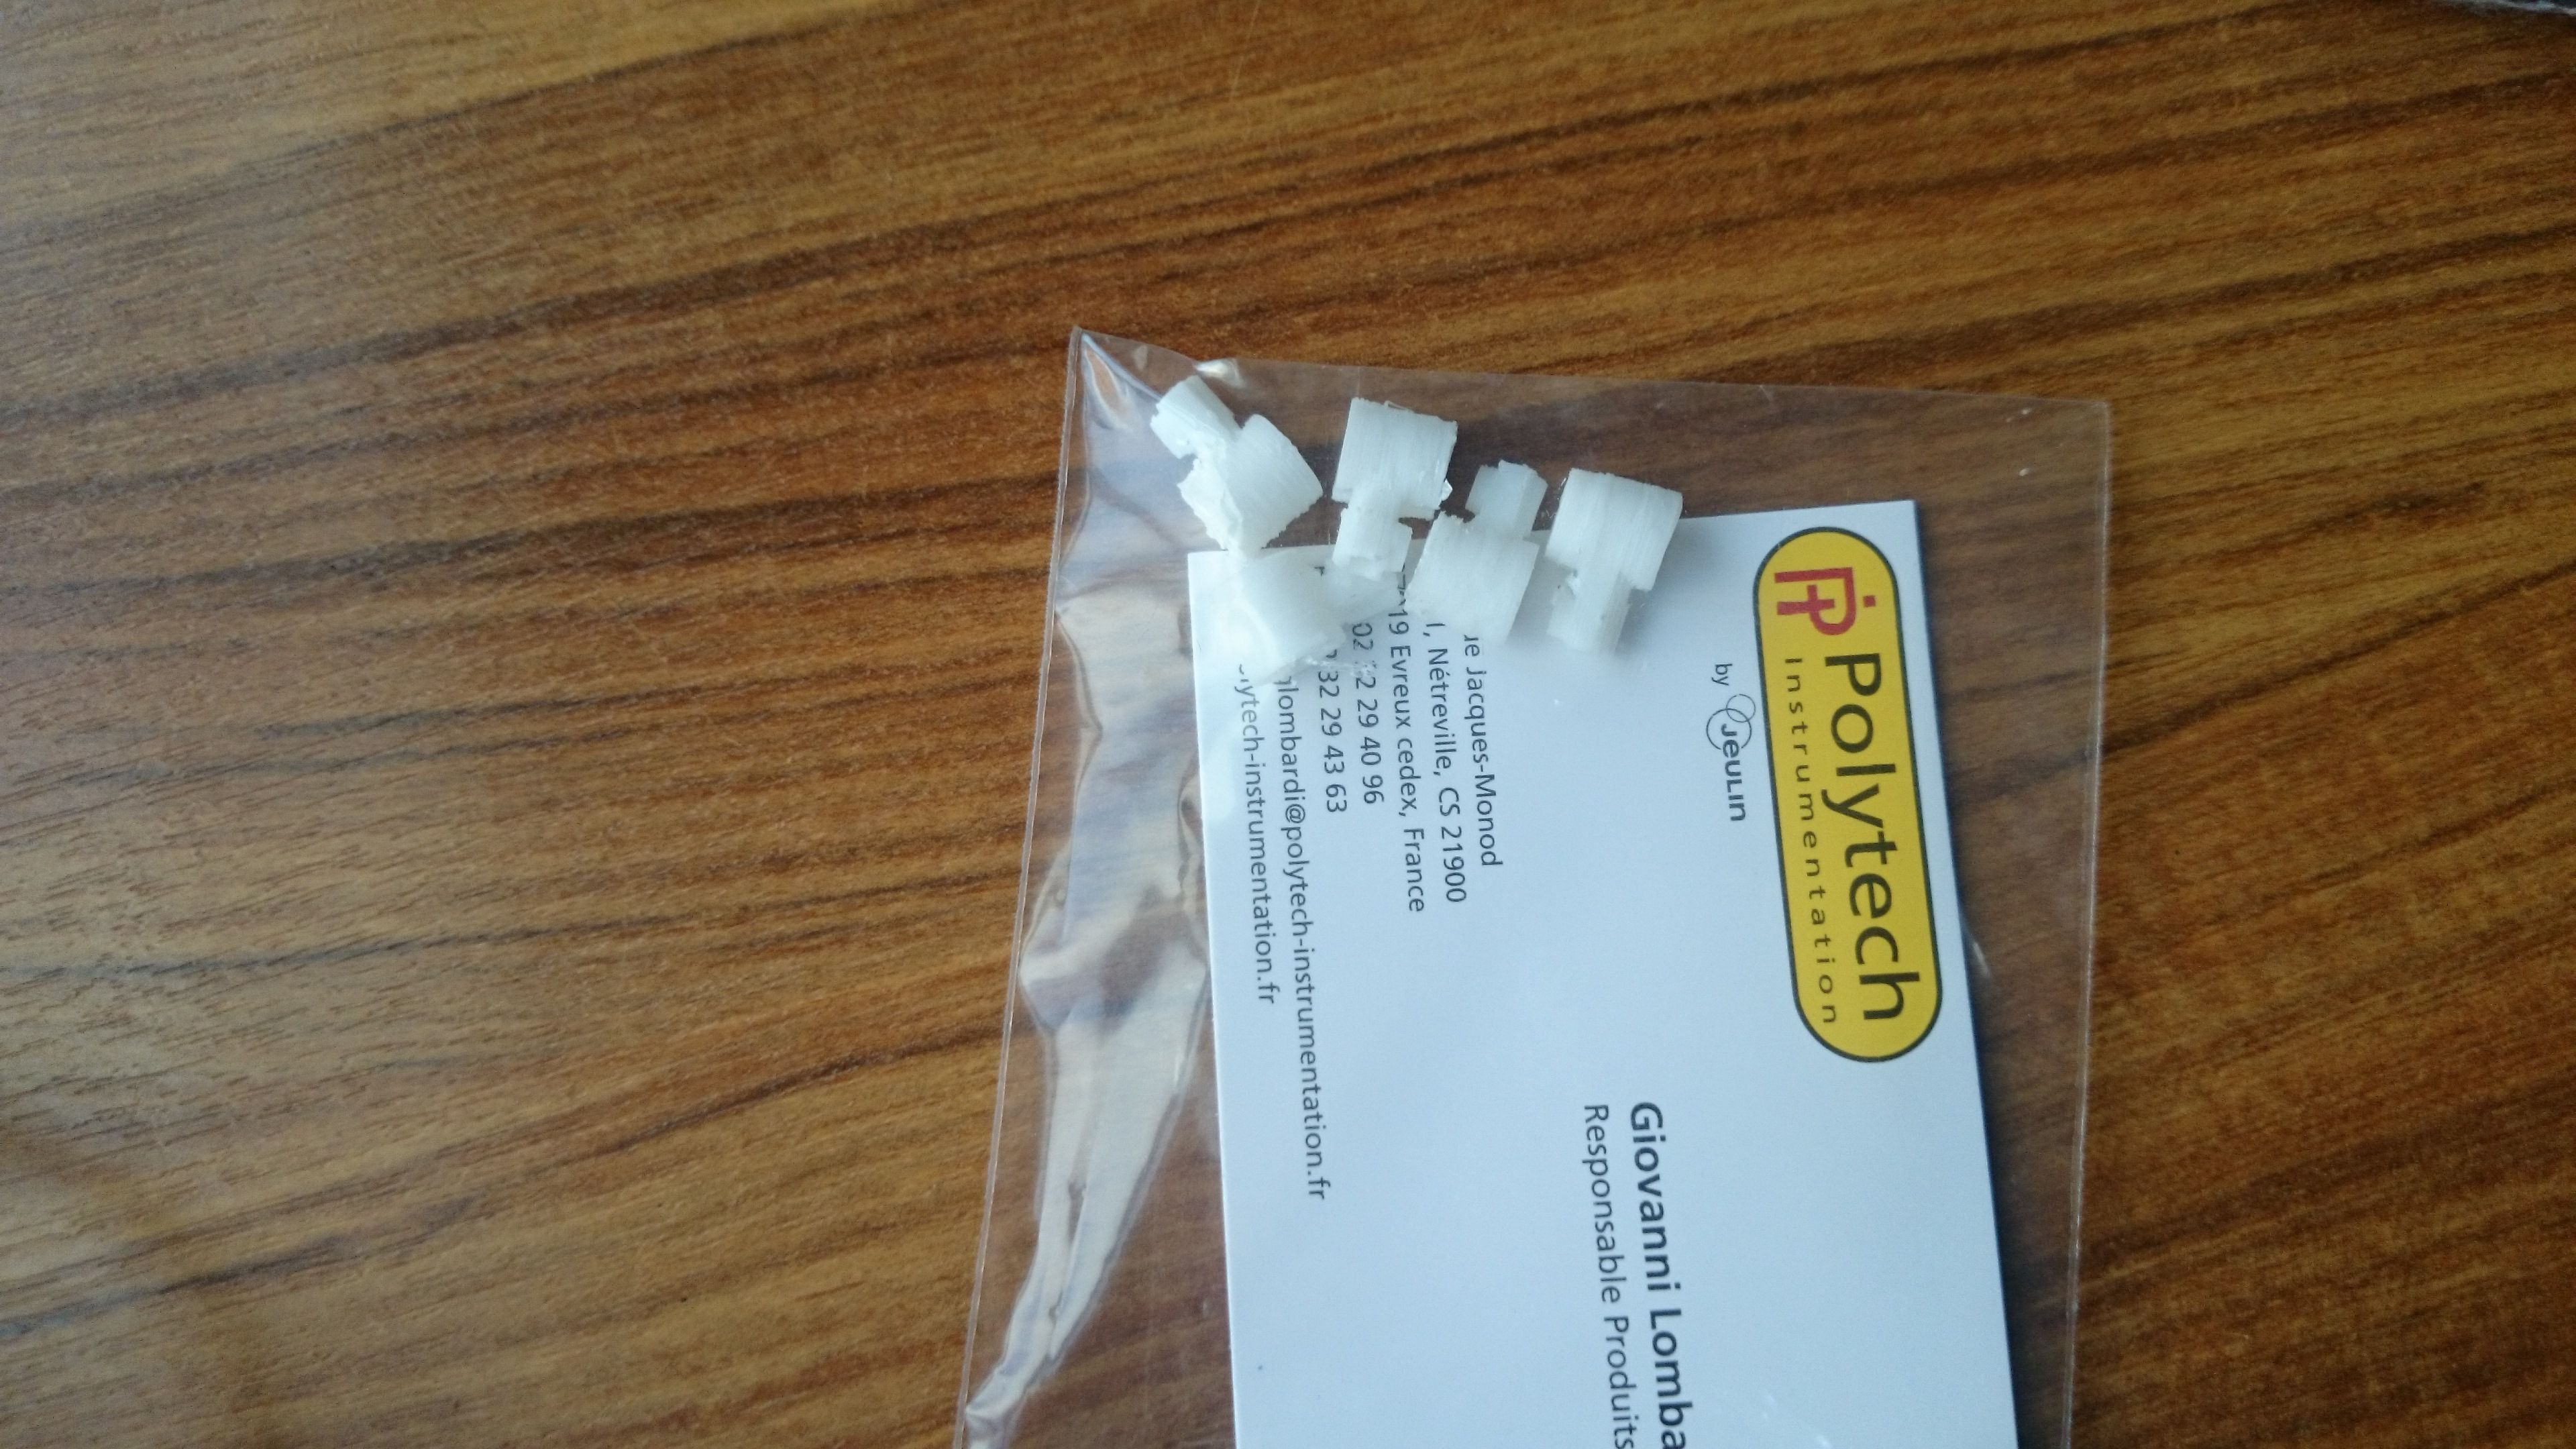
\includegraphics[scale = 0.1]{img/fixations.jpg}
	\caption{Photographie des fixations moteur}
	\label{fixation}
      \end{figure}

      Une fois les fixations moteur en notre possession, il ne nous manquait 
plus que le circuit pour assembler le tout. Pour la production de ce dernier 
nous avons eu l'idée de nous tourner vers l'\textit{ENSEA} qui est une école 
d'ingénieur en électronique proche de la nôtre. Nous leur avons fournit les 
fichiers générés par Fritzing puis ils ont lancé la production. Quelques jours 
plus tard nous avons pu aller récupérer notre circuit. Cependant, il restait 
encore quelques modifications à faire dessus, afin qu'il soit vraiment 
opérationel. En effet, il fallait encore le découper afin d'y créer des embouts 
pour les fixations moteurs. Pour cela nous avons fait appel à une connaissance 
qui dispose des outils nécessaires pour ce genre de situations. Il en a aussi 
profité pour retravailler un peu, à l'aide d'une fraiseuse, les fixations qui 
étaient un peu trop petites. La Figure \ref{circuit} est une photographie de 
notre carte avant et après découpe.

	\begin{figure}[htbp]
	  \begin{subfigure}{.5\textwidth}
	    \centering
	    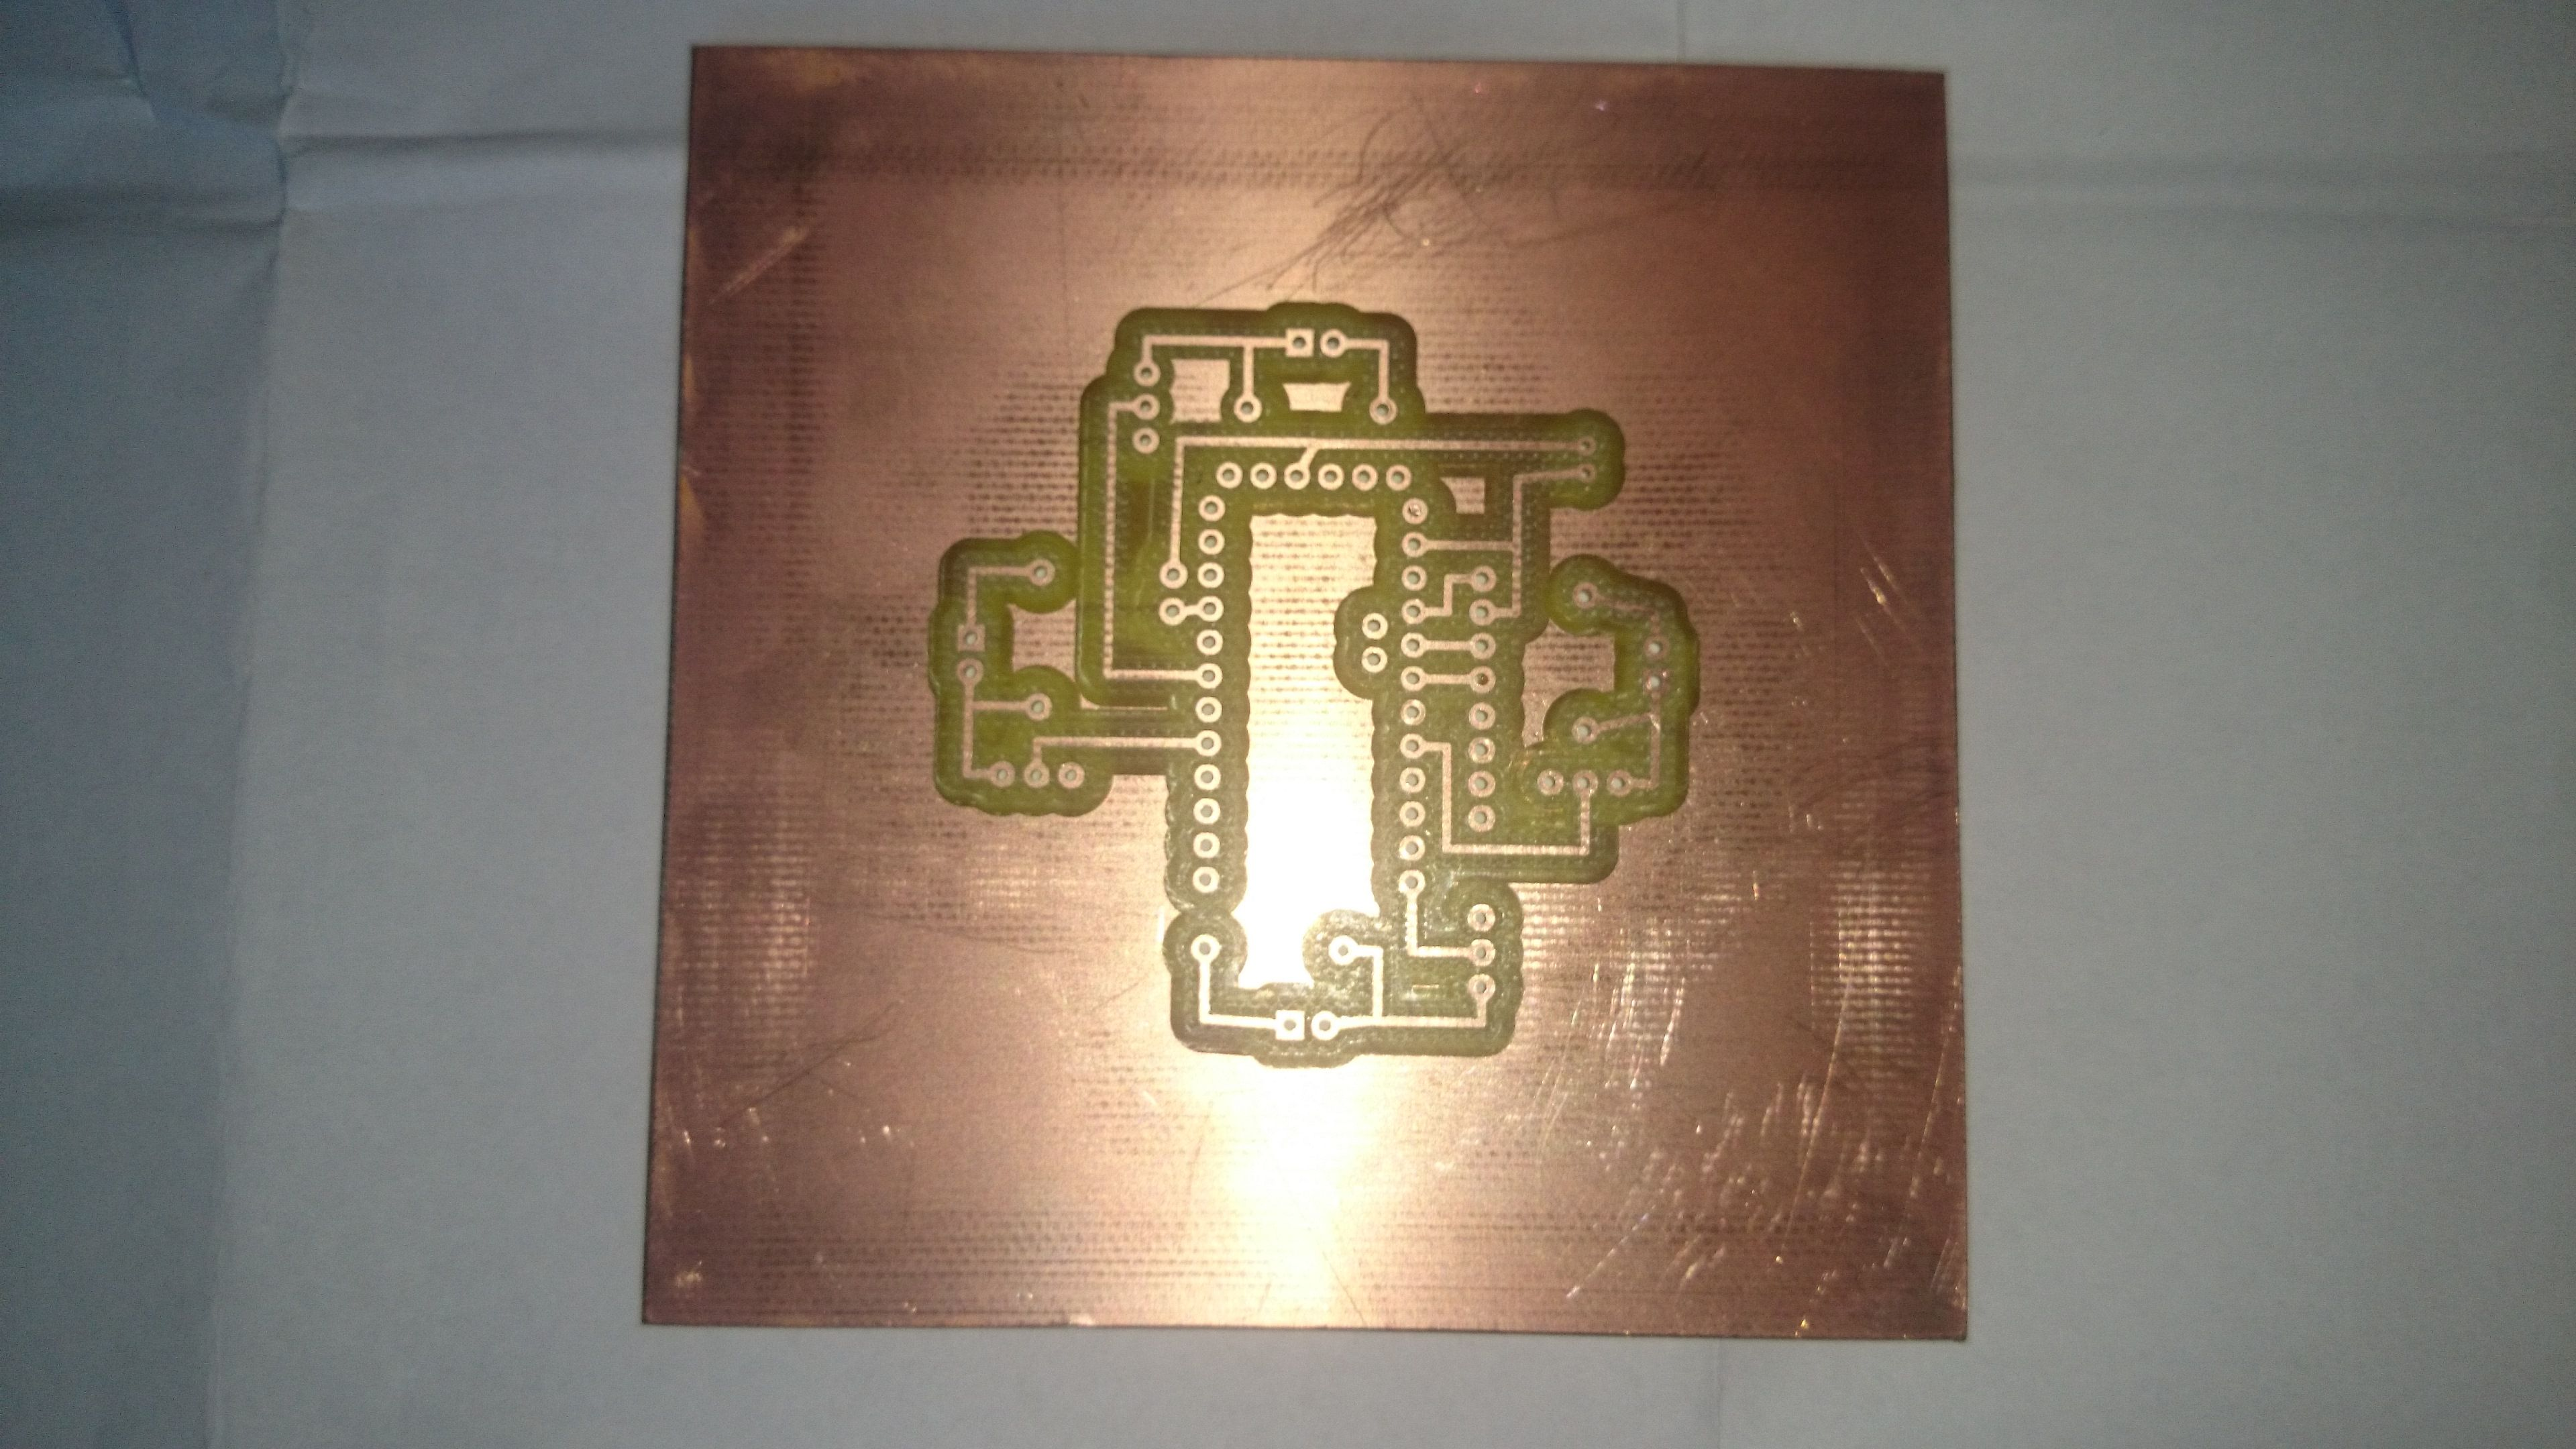
\includegraphics[scale=0.07]{img/carte_avant.jpg}
	    \caption{avant}
	    \label{circuitavant}
	  \end{subfigure}%
	  \begin{subfigure}{.5\textwidth}
	    \centering
	    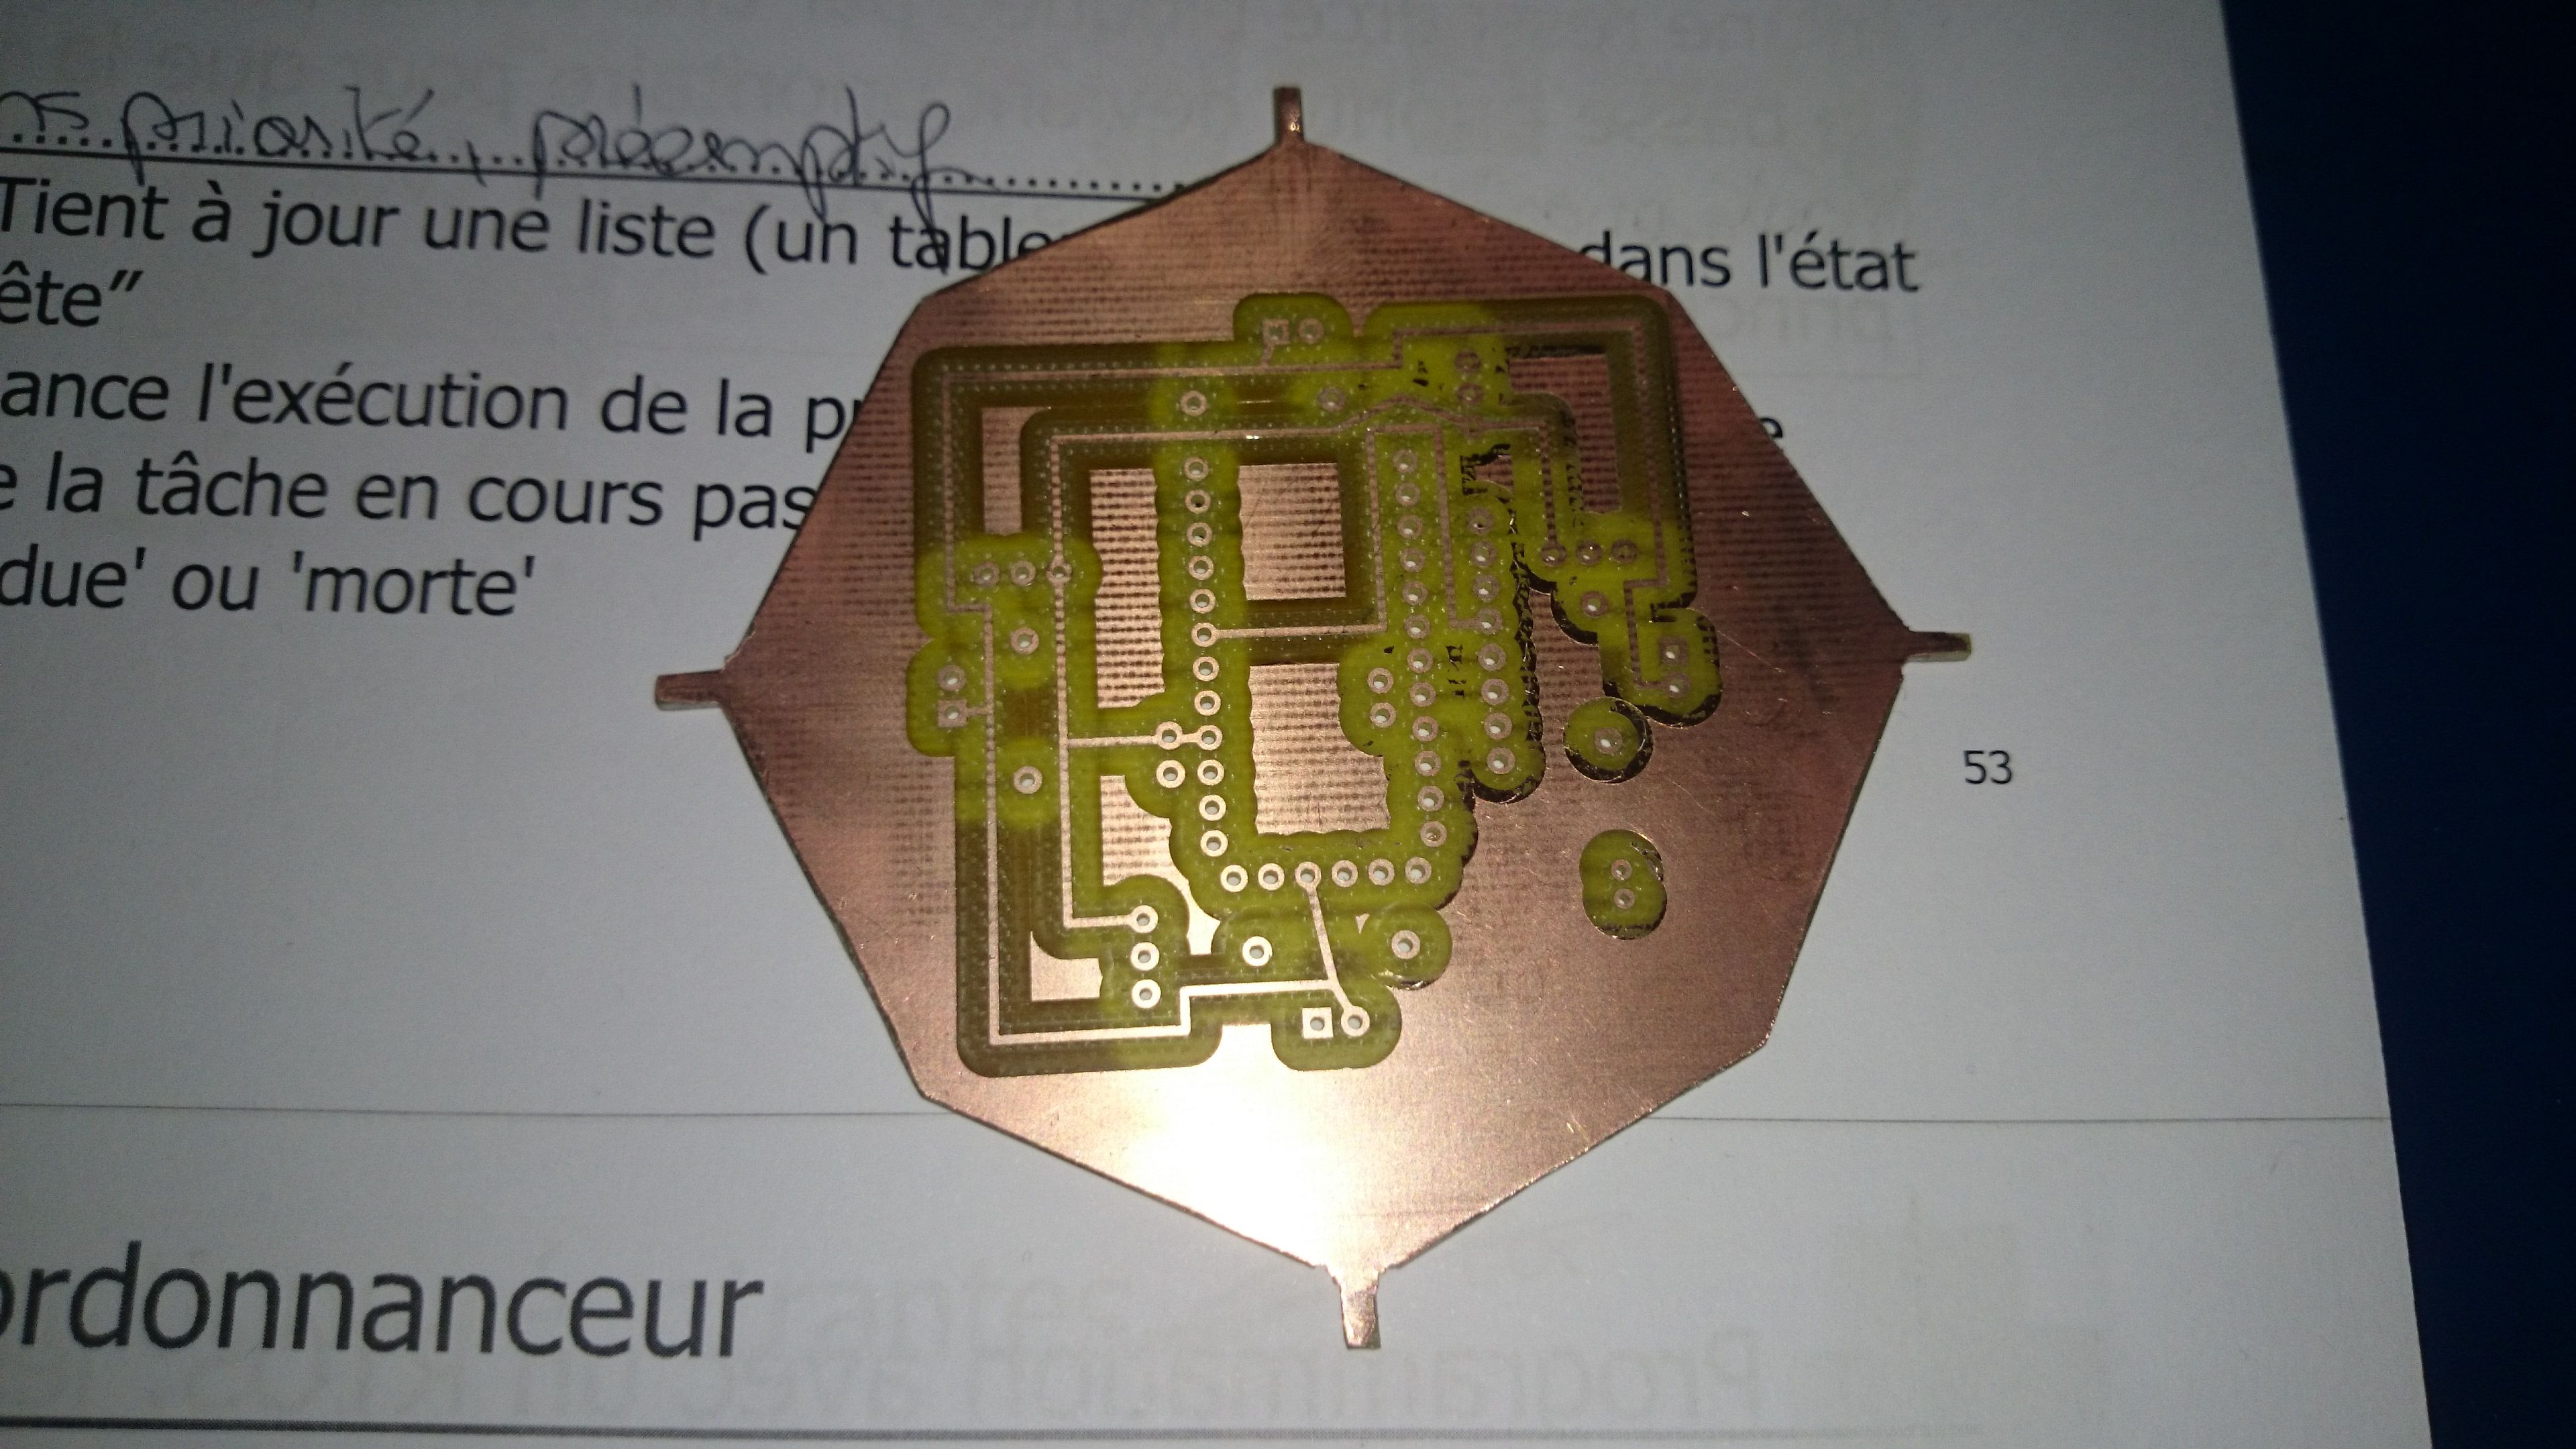
\includegraphics[scale=0.07]{img/carte_apres.jpg}
	    \caption{après}
	    \label{circuitapres}
	  \end{subfigure}
	  \caption{Photographie de notre circuit avant et après découpe}
	  \label{circuit}
	\end{figure}
      
	\subsection{Fabrication et premiers essais}
	  Une fois les deux pièces manquantes rassemblées nous avons pu passer 
à l'assemblage du drone. Nous avons donc soudé les composants sur le circuit et 
collé les fixations. Il est important de noter qu'au moment de l'assemblage 
nous avons constaté que l'Arduino que nous avions achetée n'était pas conforme 
au modèle officiel. En effet, les broches de l'alimentation étaient inversées. 
Par conséquent, notre circuit ne pouvait pas fonctionner. Nous avons dû 
racheter d'urgence une Arduino (cette fois-ci, officielle). Ce problème nous 
aura fait perdre une semaine de travail. La Figure \ref{droneres} est une 
photographie du résultat final.

	  \begin{figure}[htbp]
	    \centering
	    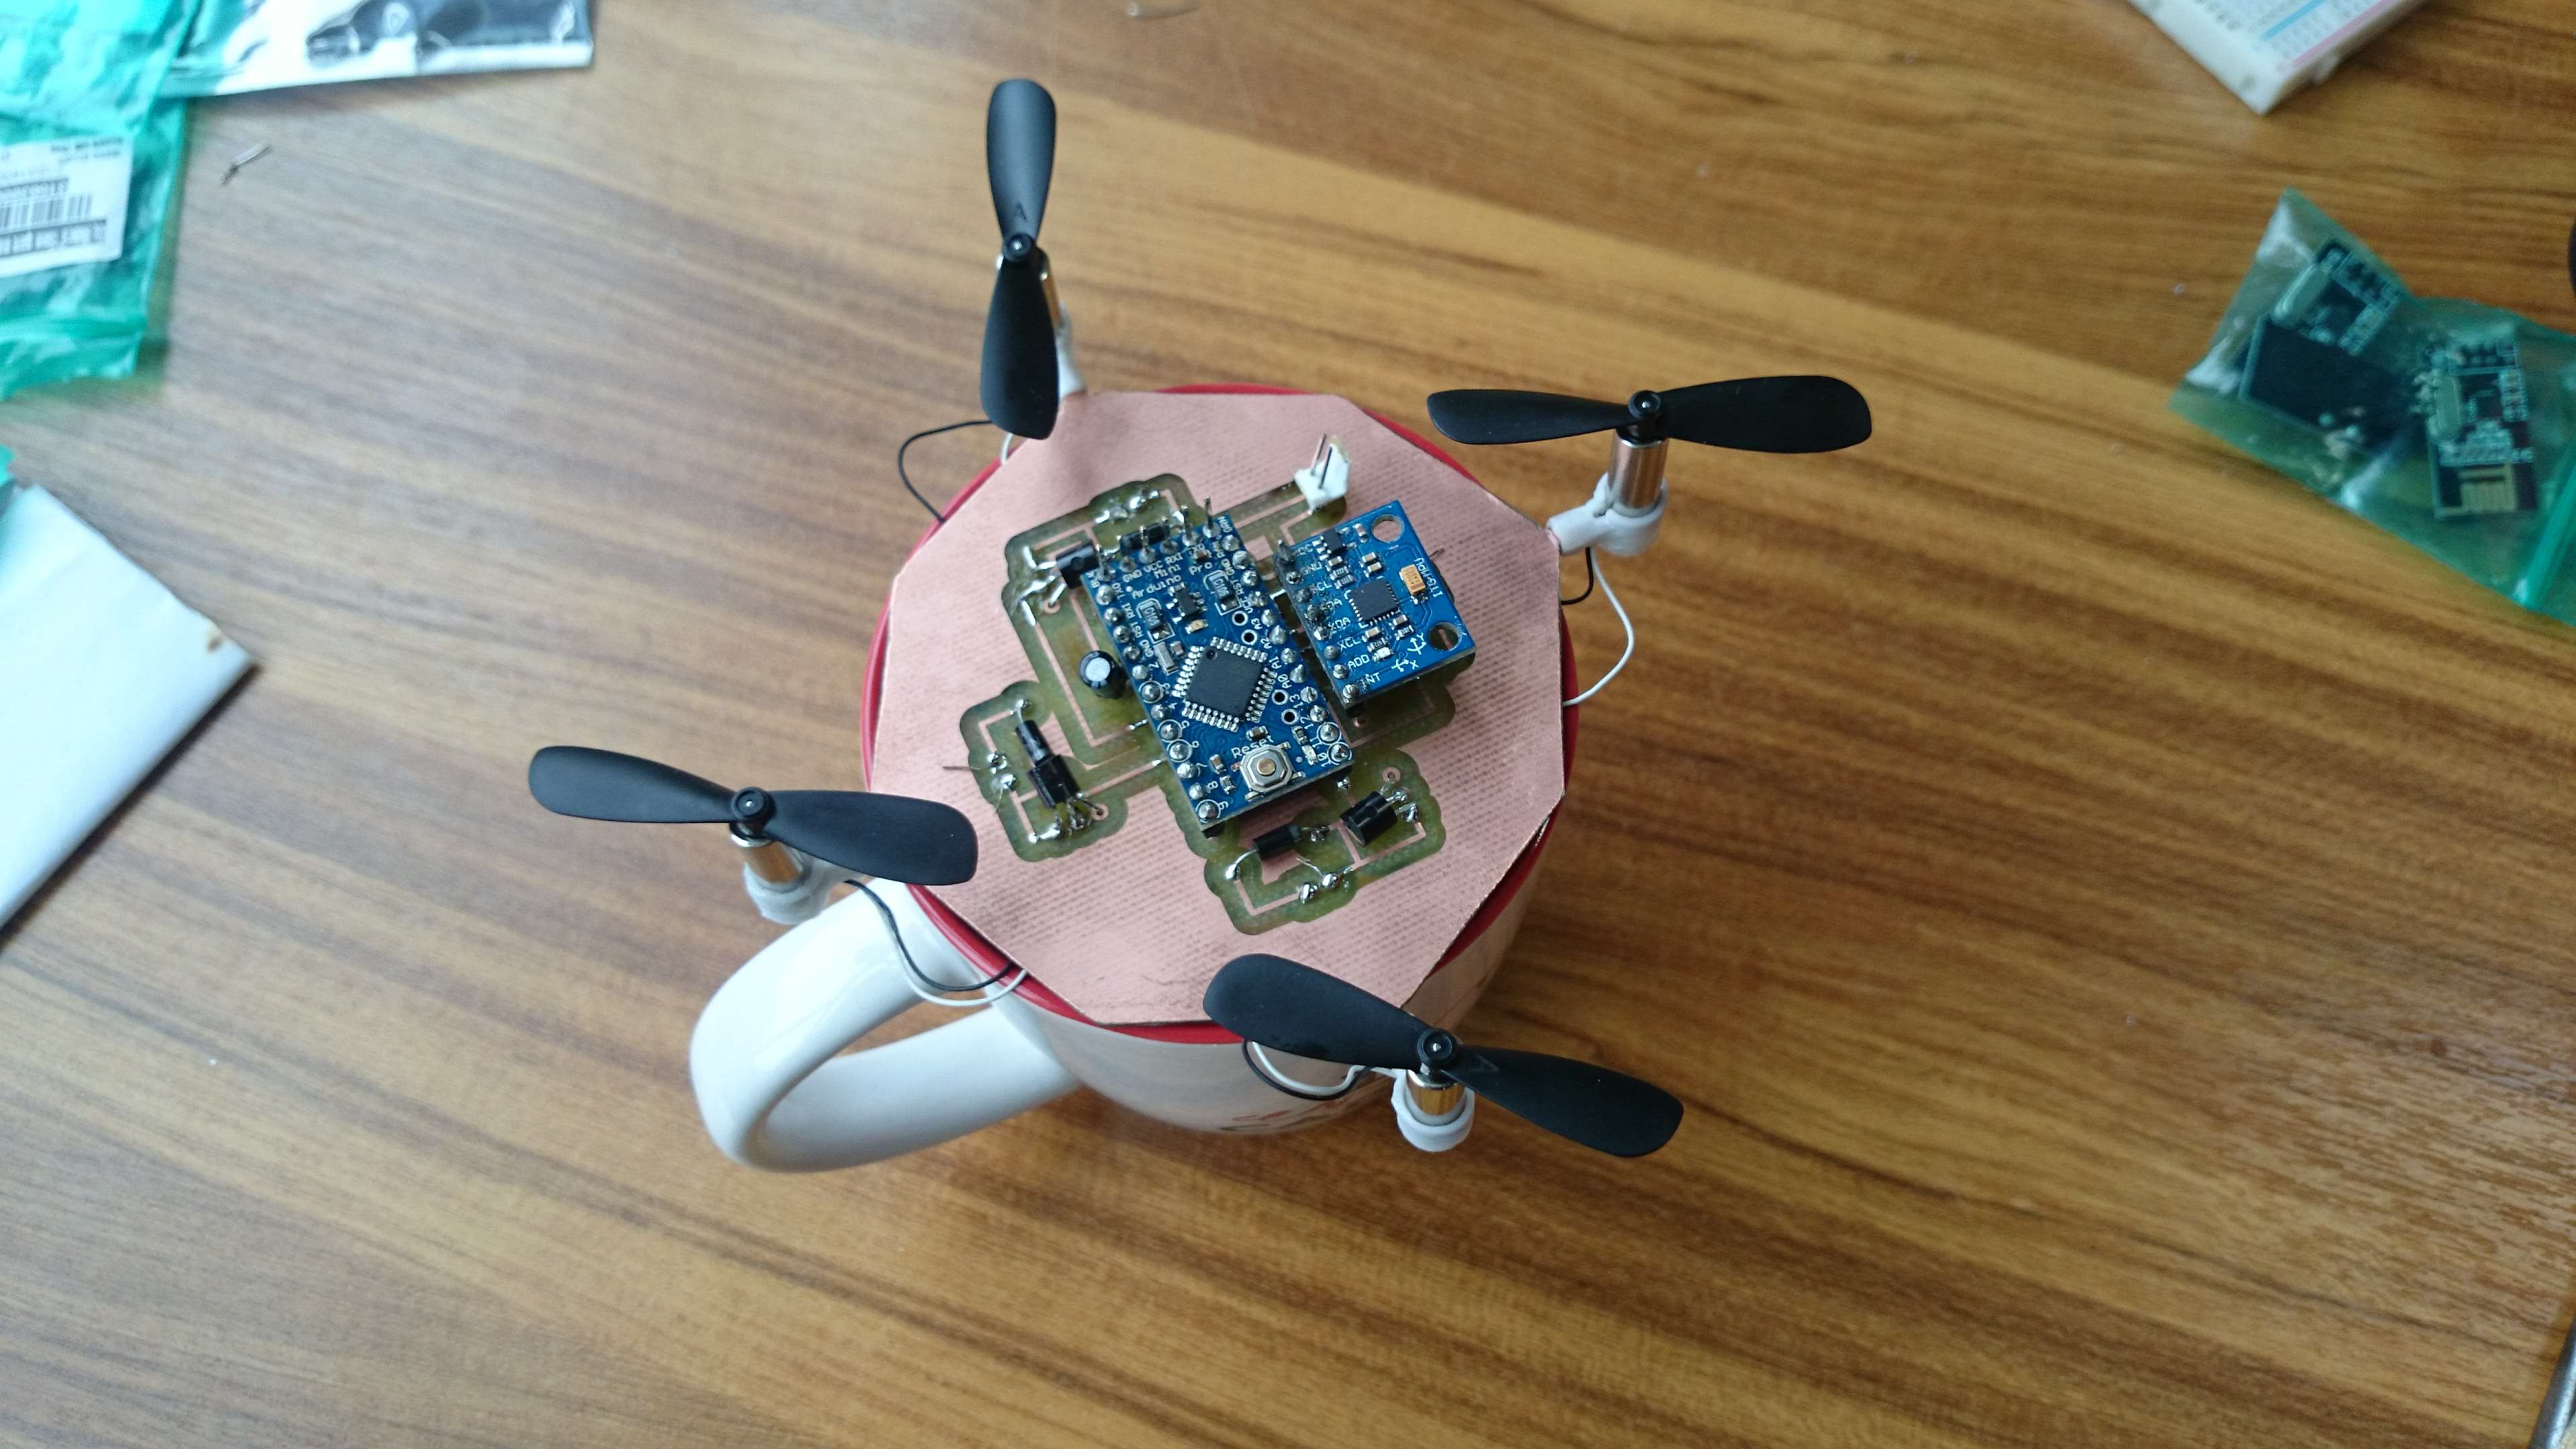
\includegraphics[scale = 0.1]{img/drone_photo.jpg}
	    \caption{Photographie du résultat final}
	    \label{droneres}
	  \end{figure}
	
	
	Une fois l'ensemble de ces étapes effectuées, il était donc possible de 
tester notre drone. Notre premier réflexe étant bien évidemment de nous assurer 
que ce dernier serait en mesure de décoller. Après diverses expérimentations, 
il s'est avéré que les moteurs n'étaient pas en mesure de tourner à plein 
régime. En effet, lorsque notre contrôleur (c'est-à-dire l'Arduino) délivre sa 
puissance maximale, les moteurs n'atteignent pas leur maximum de rotation. En 
d'autres termes, l'Arduino n'est pas en mesure de délivrer assez de courant 
pour faire tourner les moteurs au maximum de leur capacité. Le drone n'a donc 
pas décollé.

	Afin de tester un éventuel décollage du drone, nous avons décidé de 
faire un "by-pass" de l'Arduino. C'est à dire brancher les moteurs directement 
sur l'alimentation. En procédant de cette façon les moteurs tournent bien au 
maximum de leur capacité, toutefois, nous ne sommes pas en mesure de contrôler 
leur vitesse. Grâce à cette étape intermédiaire, nous avons pu constater qu'un 
des moteurs présentait un défaut, et n'était pas capable de délivrer la même 
puissance que les autres moteurs. Ainsi, lors de notre essai, le drone s'est 
soulevé d'un côté mais le manque de couple produit par le moteur défectueux à 
fait que le drone s'est retourné.

	  En analysant l'ensemble de ces problèmes, il semble raisonnable de 
penser que la présence de quatres moteurs en bon état, et tournant à leur 
maximum de puissance seraient capable de faire décoller notre drone. Toutefois, 
l'absence de contrôle sur la vitesse des moteurs nous empêcherait de contrôler 
leur vitesse, limitant notre drone à des déplacement verticaux. Nous ne 
pourrions pas le faire avancer ou aller sur les côtés. De plus nous serions 
dans l'incapacité de le faire s'arrêter.

	  Nous avons alors compris que nous ne pourrions pas faire décoller ce 
prototype. De plus, la soutenance approchait à grand pas. Nous n'étions qu'à 
deux semaines de la présentation alors nous n'avions pas le temps de préparer 
un second drone à partir d'autres composants. Nous avons toutefois préparé un 
code pour la présentation, qui servait à montrer l'influence du gyroscope sur 
le contrôle des moteurs. Lorsqu'on incline le drone, on peut voir que certains 
moteurs réagissent à cette inclinaison afin d'essayer le stabiliser. Par 
exemple, si on penche le drone vers l'avant, les moteurs avant vont accélérer 
afin d'essayer de replacer le drone parallèlement au sol. Aussi, on peut 
remarquer que plus l'angle d'inclinaison est important, plus les moteurs 
accélèrent afin de produire plus de puissance pour essayer de redresser 
l'appareil.

  \chapter{Analyse}
    Le but de ce chapitre est de faire une analyse complète de nos erreurs et 
des problèmes que nous avons rencontrés. Cette analyse pourra alors nous servir 
de point de départ pour la mise en place d'un nouveau drone. Dans n'importe 
quel projet il est important de faire le point sur les erreurs commises afin de 
ne plus les reproduire à l'avenir.

    Cette analyse parcourera l'ensemble des étapes du projet, allant de nos 
premières réflexions jusqu'à l'assemblage de l'appareil, en passant par les 
problèmes qui ne dépendent pas de nous mais de nos fournisseurs.

    \section{Conception}
      Dans cette section nous allons aborder les erreurs commises dès la 
conception du drone. C'est à dire lorsque nous avons fait le choix de nos 
composants.

      \subsection{Poids}
	Comme expliqué dans le chapitre 2, nous avons choisi de nous inspirer 
du Crazyflie. Ce drone a un type de vol très rapide et agile, alors que nous 
souhaitions que notre drone ait un type de vol plutôt hybride. Nous avons 
choisi les mêmes moteurs que le Crazyflie, mais le reste des composants étaient 
différents. En choisissant nos composants nous avons aussi calculé la somme du 
poids de chaque composant. Cependant, afin de connaître le poids total de 
notre drone nous avons dû estimer le poids de certains éléments (comme les 
transistor, les diodes, les soudures, le circuit, etc...). Pour cela nous avons 
pensé que le poids de ces éléments ne dépasserait pas 10\% de la somme calculée 
précédemment. Nous arrivions donc à un poids total de 35 grammes contre 19 
grammes pour le Crazyflie. Nous espérions donc que cette différence de poids 
irait à notre avantage, en ramenant le vol du drone à celui que nous 
attendions.
	L'erreur que nous avons commise à ce moment là, c'est d'avoir confiance 
en nos choix. Les moteurs du Crazyflie ont une documentation vraiment très 
pauvre. À tel point que leur puissance n'est même pas mentionnée. Les 
acheter en espérant que leur couple serait suffisant était vraiment une erreur 
naïve de notre part.
	Comme nous avons pu le constater lors de nos premiers essais, le couple 
de ces moteurs ne suffit pas si l'on passe par l'Arduino car notre drone est 
beaucoup trop lourd. Par contre il semble suffire s'ils sont directement reliés 
à l'alimentation. Nous en avons donc conclu que nous aurions dû choisir des 
moteurs plus puissant.
      
      \subsection{Alimentation}
	Après avoir commandé l'ensemble de nos composants nous nous sommes 
rendu compte d'un problème au point de vu de l'alimentation. Les moteurs du 
Crazyflie nécessitent une alimentation 3.3V. Nous avons établit le fait que 
l'ensemble de notre circuit serait alimenté en 3.3V. Nous avons donc choisi la 
même batterie que le Crazyflie, l'Arduino Pro Mini dans sa version 3.3V (et non 
5V), etc... Cependant nous nous sommes aperçu, par la suite, que les capteurs 
ultrasons que nous avions en notre possession demandait une alimentation de 5V. 
Ainsi, nous savions que le premier drone que nous allions construire ne 
pourrait pas nous permettre de faire l'application que nous avions prévue. Nous 
aurions pu éviter ce problème en achetant que des composants fonctionnant en 5V 
(et donc en choisissant une batterie autre que celle du Crazyflie). Nous 
aurions pu garder les moteurs que nous avions choisis, il aurait juste fallu 
créer un pont diviseur de tension\cite{pontdiviseur} à l'entrée de chaque 
moteur. Un pont diviseur de tension est un montage de deux résistances, très 
simple à mettre en place, permettant de réduire une tension. Ainsi nous aurions 
pu avoir un circuit qui fonctionne en 5V, sauf à l'entrée des moteurs où cette 
tension aurait été réduite à 3.3V.

	Nous avons tout de même pensé qu'il serait intéressant de monter ce 
premier drone tout en sachant qu'il ne pourrait pas remplir notre cahier des 
charges. En effet, nous avons pensé qu'il pourrait nous permettre de vérifier 
nos calculs (autonomie de la batterie, poussé des moteurs, puissance requise, 
...). Finalement, les résultats de nos calculs étaient plutôt proche de la 
réalité. Nous avions estimé l'autonomie de la batterie à sept minutes. Et en 
réalité elle se décharge en cinq minutes en faisant tourner les moteurs à plein 
régime. Cependant, il est important de noter qu'il n'y a ni les capteurs 
ultrasons ni le transmetteur/récepteur radio. L'autonomie est donc trop courte 
pour notre application. Aussi, lorsque les moteurs tournent à plein régime on 
peut remarquer que le drone se soulève et que ce qui l'empêche de décoller est 
le moteur défectueux. On peut donc en conclure que nos calculs mécaniques 
étaient plutôt bons. Vous pouvez retrouver ces calculs dans l'Annexe C de ce 
rapport.
    
    \section{Fournisseurs}
      Le rôle de cette section est de présenter les problèmes venant des 
différents fournisseurs et qui donc ne dépendent pas de nous.
      \subsection{Délais}
	Comme nous l'avons expliqué précédemment, notre école étant une école 
d'informatique est donc peu adaptée à des projets qui ont pour objectif de 
faire une réalisation matérielle. Nous avons alors eu besoin d'un support 
extérieur pour les fixations moteur, la réalisation du circuit imprimé et sa 
découpe. Mais la recherche de ces entités prend un certain temps, auquel il 
faut ajouter le temps de création des éléments. Nous arrivons alors à un délai 
conséquent, qui peut prendre plusieurs mois suivant l'entité. Par exemple si 
l'on passe par un fablab, il faut ajouter à cela le temps qu'il faut pour 
apprendre à se servir des machines. En ce qui nous concerne nous avons eu un 
peu de chance en rencontrant Polytech Instrumentation. Car sans eux nous 
aurions peut-être pris encore plus de temps pour trouver des imprimantes 3D. 
De plus, il est important de noter que le temps de réception des différents 
composants électroniques prend un temps considérable (de l'ordre d'un mois). 
Parfois ce temps peut être utilisé pour avancer d'autres parties du projet 
(comme le serveur). Mais dans l'autre cas, c'est du temps de perdu car nous 
avons besoin des composants pour apprendre à nous en servir, développer leur 
librairie et donc tout simplement avancer dans le projet.

	Nos premiers essais ont été fait fin février. La soutenance étant 
prévue pour le 16 mars, cela nous a laissé deux semaines de marge. Cependant, 
ce laps de temps est loin d'être suffisant pour concevoir un second drone. 
Ainsi, nous n'avons pas pu profiter de l'expérience acquise tout au long du 
projet, pour mettre en place une seconde version du drone. Nous pensons alors 
que les premiers essais auraient dû être fait fin 2014 pour nous laisser le 
temps de produire un drone fonctionnel. Malheureusement, le projet de fin 
d'étude, commençant en septembre, cela ne laisse que quatre mois pour produire 
un premier drone. Ce qui est un délai vraiment trop court. Ainsi, nous pensons 
qu'une telle application ne peut pas être faite en sept mois, avec nos moyens.
      
      \subsection{Fiabilité}
	Un des avantages d'Arduino (et du Crazyflie) est que ce soit un projet 
libre. Cependant, ceci peut devenir un désavantage. En effet, n'importe qui 
peut produire les composants. Ainsi il est possible d'acheter des composans à 
un prix vraiment faible comparé aux fournisseurs officiels. Mais, il n'existe 
aucune garantie de fiabilié si on ne passe pas par ces fournisseurs et bien 
trop souvent ce coût réduit se ressent sur la qualité des composants.
	
	Par exemple, nous pouvons citer les problèmes d'Arduino que nous avons 
rencontrés. Après avoir reçu tous les composants commandés, l'Arduino manquait 
toujours à l'appel. Ainsi après avoir attendu plus de deux mois, nous avons 
recontacté le vendeur qui nous a assuré que le composant était arrivé chez 
nous. Nous avons alors demandé un remboursement et commandé chez un autre 
fournisseur. Aussi, comme nous l'avons expliqué précédemment, lors de 
l'assemblage du drone, nous nous sommes rendus compte que l'Arduino que nous 
avions commandé n'était pas une "Arduino Pro Mini" mais une "Arduino Mini Pro" 
(donc une contrefaçon). Et les broches de l'alimentation étaient inversées, ce 
qui faussait tout notre circuit.

      Nous pouvons citer un autre exemple, les quatres moteurs que nous avons 
achetés proviennent du même fournisseur. Cependant, il y a un moteur défectueux 
dans le lot.

      Un dernier exemple en citant le manque de qualité du côté des composants 
radio. Nous ne pouvons recevoir tous les messages envoyés (de l'ordre de un 
message sur deux). Si nous utilisions ces composants dans une application 
réelle nous ne pourrions pas parler d'une transmission fiable. De plus cela 
pourrait être dangereux, si par exemple on demandait à un drone de se poser et 
qu'il ne recevait pas le message. Il est important de noter qu'au début du 
développement de la librairie, la fiabilité était encore plus médiocre. Mais en 
recherchant sur Internet, nous avons vu des sites webs qui expliquaient qu'il 
faut brancher un condensateur entre les deux broches de l'alimentation. Le 
fournisseur vend donc un produit qui n'est pas du tout fiable.

      Ainsi, nous avons compris que faire des économies peut être un avantage 
(nous avons pu monter un drone pour un peu moins de 30 \euro, tandis que le 
Crazyflie vaut environ 120 \euro). Mais à vouloir trop chercher le moins cher, 
on prend des risques sur la qualité des produits. Il faut donc mieux 
rechercher, se méfier de la contrefaçon et faire plus d'essais lors de la 
réception des pièces.
    
    \section{Assemblage}
      En ce qui concerne l'assemblage, il y a une problématique que nous 
n'avons pas prise en compte au moment de la conception. En effet, en 
choisissant les moteurs du Crazyflie, nous étions dépendant de leur dimension 
atypique. Aussi, les moteurs de drones possèdent généralement des pas de vis 
afin d'être vissés au châssis. Ce qui n'est pas le cas des moteurs que nous 
possédons. Ainsi, nous avons plus ou moins été contraints d'utiliser le même 
système de fixation que le Crazyflie. Cependant, nous avons omis le fait que le 
Crazyflie est assemblé par des machines et que pour notre drone c'est nous qui 
allions devoir le monter. Or, les machines peuvent placer des éléments avec un 
degré de précision proche de la perfection, ce qui n'est pas le cas de l'être 
humain. Donc, outre le fait que nos fixations risquaient de ne pas être 
parfaitement fiables (les imprimantes 3D étant une technologie assez récente) 
nous serions incapable de fixer les moteurs parfaitement verticaux. Ce qui 
entraînerait un défaut dans le vol de l'appareil. En effet, si un moteur était 
penché plus d'un côté que les autres, cela produirait une dérive dans la 
direction du drone. Aussi, suivant le défaut d'inclinaison des moteurs, cela 
peut entraîner une perte de poussé des moteurs et donc rendre le décollage de 
l'appareil plus difficile.
    
    \section{Expérience}
      Il est important de noter le côté ambitieux de notre projet. En effet, 
nous avons jusqu'à cette année suivi une formation orientée dans l'ingénerie 
informatique. En nous spécialisant dans l'informatique embarquée, nous avons 
mis un pied dans l'ingénerie système. Cependant, nous ne sommes pas des 
ingénieurs système. Ainsi même pour des personnes de cette profession, un tel 
projet nécessite plusieurs années.

      De plus nous avons eu affaire à des contraintes et réfléchir à des 
problématiques auxquelles nous ne sommes pas habitués (comparer du matériel, 
prendre en compte des délais de livraison, contraintes système telles que la 
tension, le courant, le poids, la puissance délivrée...). Nous avons commis 
beaucoup de petites erreurs pour cette raison, mais si nous devions réfléchir à 
une seconde version nous serions probablement mieux préparé car nous avons 
beaucoup appris de ces erreurs.
  
  \chapter{Deuxième drone}
    Bien que le temps ne nous permette pas de réaliser un second drone, nous 
pouvons tout de même établir un nouveau devis afin d'utiliser une partie de 
l'expérience que nous avons acquise.

    Pour rappel, les principaux problèmes de notre premier drone sont :
    
      \begin{itemize}
	\item Moteurs pas assez puissants
	\item Voltage du circuit
	\item Autonomie de la batterie
      \end{itemize}
      
   Pour ce second drone nous changerons donc les moteurs et la batterie. Nous 
garderons par contre les autres composants qui malgré leur manque de fiabilité 
suffirait pour une simple présentation. Bien entendu, pour une application 
réelle il faudrait voir à choisir des composants de meilleure qualité.

    \section{Moteurs}
      Le problème de nos moteurs actuels est le couple maximum qu'ils peuvent 
fournir. En effet, celui-ci est sur la limite de ce dont notre drone à besoin. 
Ainsi, à plein régime ils pourraient peut-être suffire, mais nous ne pourrions 
pas vraiment jouer sur leur vitesse de rotation. 

      C'est pour cette raison que nous avons cherché des moteurs plus 
puissants. Nous avons alors choisi les \textit{DYS BE1806-13} (voir Figure 
\ref{dys}). Ces moteurs n'ont plus rien avoir avec ceux que nous avions avant 
puisqu'ils sont environ trois fois plus gros et douze fois plus lourd. Ceci va 
entraîner un changement radical dans la dimension de notre drone. En fait, un 
drone de la dimension du Crazyflie n'est pas forcément un bon point de départ 
pour des débutants comme nous car les composants sont assez spécifiques. Ainsi, 
en nous ramenant à une dimension plus "standard", nous élargissons notre 
catalogue de composants. Ce deuxième drone devrait alors faire environ 30 
centimètres de diamètre pour un peu moins de 370 grammes.

      \begin{figure}[htbp]
	\centering
	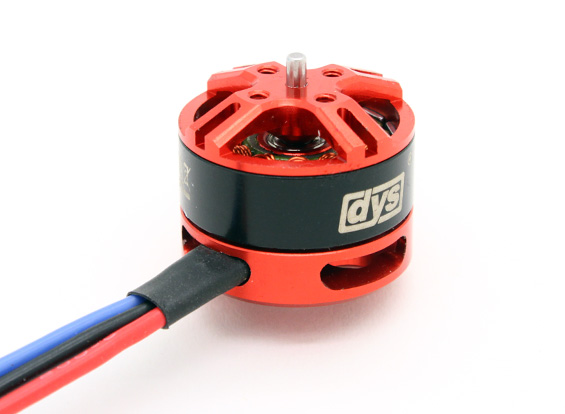
\includegraphics[scale = 0.25]{img/dys.jpg}
	\caption{Image d'un moteur DYS BE1806-13}
	\label{dys}
      \end{figure}

      Pour ces moteurs nous disposons d'une documentation assez complète. 
Ainsi, nous sommes capables de faire nos calculs sans faire d'estimation. Ces 
moteurs sont capables de fournir une puissance maximum de 89 watts. Pour un 
drone de 370 grammes il faut compter une puissance 9 watts par moteur. Nous 
pouvons donc remarquer que les moteurs choisis sont bien supérieurs à ce que 
le drone requiert. Mais, cela nous permettrait d'avoir une grande marge de 
manoeuvre sur la vitesse de rotation des moteurs. Aussi, cela nous permettrait 
d'éviter de faire tourner les moteurs à plein régime de manière constante, ce 
qui augmenterait leur durée de vie et qui déchargerait moins vite la batterie.

      Dû aux nouveaux moteurs qui sont beaucoup plus puissants et à la 
nouvelle dimension de notre drone, il nous faut choisir de nouvelles pales 
(plus longues). Nous avons alors choisi des \textit{APC 6*2 .049} (voir Figure 
\ref{pale}). Ces pales font six pouces de longueur (environ 15 centimètres).

      \begin{figure}[htbp]
	\centering
	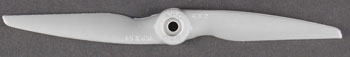
\includegraphics[scale = 0.4]{img/pale.jpg}
	\caption{Image d'une pale APC 6x2 .049}
	\label{pale}
      \end{figure}
      
      Grâce à ces nouvelles pales plus longues, le drone pourra plus facilement 
brasser l'air et donc décoller plus facilement. Par contre, nous perdrons en 
vitesse, mais pour rappel, nous cherchons justement à obtenir un vol hybride 
afin d'obtenir le plus d'informations possible sans être lent au point de 
pouvoir faire des prises de vue.

    \section{Batterie}
      Comme nous l'expliquions dans le chapitre précédent, nous avons un 
problème de voltage sur notre premier drone. Les capteurs ultrasons ont besoin 
d'une tension de 5V, tandis que la batterie fournit du 3.3V. Il nous faut alors 
un voltage plus élevé. C'est pour cette raison que nous avons sélectionné une 
\textit{Turnigy 1700Mah 7.4v} (voir Figure \ref{batterie}). On peut remarquer 
que la tension délivrée par cette batterie est supérieure à 5V, mais comme nous 
l'avons expliqué une tension peut se réduire à l'aide d'un pont diviseur de 
tension (par contre le problème inverse est plus compliqué à résoudre).

      \begin{figure}[htbp]
	\centering
	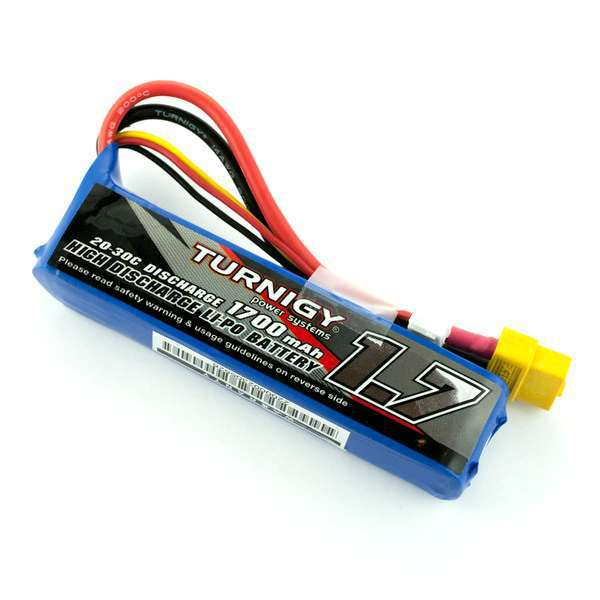
\includegraphics[scale = 0.25]{img/nouvellebatterie.jpg}
	\caption{Image d'une batterie Turnigy 1700Mah 7.4v}
	\label{batterie}
      \end{figure}

      D'après nos calculs, le drone devrait avoir besoin de 1600mA par moteur 
pour décoller et l'ensemble des autres composants demandent 124mA de manière 
continue. Ainsi, avec cette batterie qui peut fournir 1700mAh, nous devrions 
avoir une autonomie d'une quinzaine de minutes. L'autonomie de ce nouveau drone 
est donc doublée par rapport au précédent, alors qu'il doit alimenter six 
capteurs ultrasons ainsi que le transmetteur/récepteur radio (ce que ne faisait 
pas l'ancien).

    \section{Coût total}
      Ce nouveau devis nous indique un prix beaucoup plus élevé que pour le 
premier. En effet, nous arrivons à environ 75 \euro, tandis que le premier 
drone nous a coûté environ 25 \euro. Ceci s'explique notamment que le prix des 
batteries est proportionnel à leur capacité. Aussi, les moteurs du Crazyflie 
sont vraiment bon marché comparativement aux autres moteurs. Il n'est donc 
pas étonnant d'aboutir à un prix plus élevé.

      Aussi il ne faut pas oublier de changer l'Arduino Pro Mini 3.3V, en sa 
version 5V. Cependant le prix est le même entre les deux versions.
  
  \chapter{Conclusion}
    Maintenant que toutes les étapes du projet ont été abordées, nous pouvons 
conclure ce rapport.

    Nous pouvons commencer par dire que divers éléments ont été implémentés. 
Premièrement nous pouvons discuter du serveur. Celui-ci est quasiment 
fonctionnel, dans le sens où il remplit bien sa fonction première à savoir, 
dessiner la topographie de la zone étudiée. Cependant, il n'est pas entièrement 
fonctionnel puisque sa deuxième fonction, envoyer des ordres aux drones, ne 
fonctionne pas encore. En effet, le serveur arrive bien à déterminer si un 
ordre doit être envoyé puis à faire remonter cet ordre jusqu'à la première 
tâche (c'est-à-dire, écrire l'ordre sur le port série de la machine). 
Cependant, nous n'arrivons pas à faire en sorte que la première tâche écrive 
les messages des drones sur le port série puis simultanément lise les ordres 
sur le port série. Pour le moment nous ne pouvons faire seulement l'un ou 
l'autre.

    En admettant que le serveur soit fonctionnel. Il nous faudrait quand même 
un drone opérationel afin de faire de vrais essais. Ce qui nous permettrait 
alors d'établir une liste complète des états du drone qui nécessitent un envoi 
d'ordre. Car il est compliqué d'établir une liste exhaustive sans voir le 
déroulement réel de notre application. Bien sûr, nous pouvons commencer par 
penser à quelques états. Mais il est quasiment certain que nous en oublierons. 
C'est pour cette raison qu'un drone fonctionnel serait d'une grande utilité. 

    Dans un deuxième temps nous pouvons parler de la construction du drone. 
Ceci représentait un challenge énorme. En effet, ce projet requiert des 
connaissances pluridisciplinaires et complexes (mécanique, électronique, 
informatique, physique, ...). Au vu de notre formation orientée informatique, 
nous avons fait beaucoup trop de petites erreurs dans les domaines qui ne sont 
pas notre spécialisation. Ces erreurs ont conduit à un drone ne pouvant pas 
voler. Cependant, nous avons beaucoup appris de nos erreurs. Mais ce projet 
était un peu trop ambitieux. Nous ne disposions que de sept mois pour le 
réaliser, alors qu'il faudrait plutôt partir sur un ou deux ans. De plus ce 
manque de temps, ne nous a pas permis de profiter de l'expérience acquise 
durant le projet.

    Même si nous avions réussi à produire un drone qui est capable de voler. 
Nous serions encore bloqué à la problématique de la détermination de la 
position du drone dans l'espace étudié. Il plutôt simple de localiser un drone 
sur une grande étendue (c'est-à-dire, lorsque l'on ne cherche pas à obtenir une 
précision au décimètre près) en extérieur grâce au GPS. Cependant, nous savions 
que nous devrions présenter le projet dans une pièce. Ainsi, la précision d'un 
GPS n'est pas assez suffisante (de l'ordre de trois à cinq mètres). Donc, le 
GPS ne détecterait quasiment aucun déplacement. C'est pour cette raison que 
nous avons cherché d'autres solutions et que l'idée de calculer la position du 
drone en mesurant et en intégrant deux fois son accélération (à l'aide d'un 
accéléromètre) nous est venue. Cependant, chaque intégration introduit une 
erreur et dû à la double intégration, cela produit une erreur quadratique. 
Ainsi, nous serions peut-être capable de localiser à peu près le drone au début 
de l'application, mais tout au long de son déroulement l'erreur introduite par 
l'intégration fausserait complètement nos résultats. Il est important de noter 
que cette problématique est encore au stade de la recherche. Et que pour le 
moment il n'existe peu (voir pas) de moyens fiable de localiser un objet en 
mouvement avec beaucoup de précision (avec un faible coût financier et 
technique).

    Bien que ce projet n'est pu aboutir à l'objectif initialement prévu, cela a 
été un plaisir de travailler sur ce sujet. Du fait des nombreuses connaissances 
qu'il demande dans des domaines variés, nous pouvons dire que c'était un projet 
très enrichissant techniquement parlant. Et puisque nous avons dû faire appel à 
de l'aide extérieure à l'EISTI afin d'obtenir certains de nos composants, nous 
pouvons aussi dire que c'était enrichissant sur le plan relationnel. Car nous 
avons dû faire de nombreuses démarches vers des entités extérieures à notre 
école afin d'obtenir les derniers éléments qu'ils nous manquaient.

    Mais nous n'aurions peut-être pas pu réussir ces démarches sans l'aide de 
madame \textit{Nga Nguyen}, pour obtenir la participation de Polytech 
Instrumentation ni sans l'aide de madame \textit{Besma Zeddini}, pour obtenir 
la participation de l'ENSEA. C'est pour cette raison que nous souhaitons 
remercier les quatre noms cités ci-dessus, ainsi que les divers connaissances 
qui nous ont aidées dans notre projet, à savoir pour la découpe du circuit et 
pour divers conseils techniques.
   
  \appendix
    \chapter{Suivi de projet}
      \section{Gestionnaire de version}
	Pour ce projet nous avons choisi de former un groupe de trois 
personnes. Travailler en équipe a ses avantages, notamment pour le partage des 
tâches. Mais ceci peut entraîner des problèmes de versions entre les travaux de 
chacun. Pour palier ce problème nous avons choisi d'utiliser le gestionnaire 
de version Git\cite{git}. Cet outil est vraiment pratique, puisqu'il permet de 
travailler à distance, de mettre à jour le code de chacun des membres, d'avoir 
un suivi de chaque implémentation, de faire des versions tests (sans toucher à 
la version fonctionnelle) ou encore de revenir à des versions précédentes du 
projet. Aussi cet outil nous permet de donner une visibilité à notre travail. 
Ainsi, si une personne compte faire un projet semblable au nôtre il pourra 
consulter, reprendre, modifier, améliorer... ce que nous avons fait.

	Plus précisément nous avons créé une "organization"\cite{njordgit} sur 
\textit{GitHub}\cite{github}. Ceci nous a permis de décomposer l'ensemble du 
projet en plusieurs répertoires. Ainsi chacun peut accéder à la partie du 
projet qui l'intéresse sans avoir à récupérer l'ensemble de l'application. Par 
exemple si un utilisateur souhaite ne travailler que sur le drone, il peut le 
faire sans avoir à télécharger en plus la partie qui s'occupe du serveur. Aussi 
un projet bien découpé est plus compréhensible et plus facilement réutilisable. 
De plus, une "organization" peut héberger un petit site web statique. Ce qui 
nous a permis de mettre en place notre blog\cite{njordblog}. 
	
      \section{Communication}
	Dès le début du projet nous avons pensé qu'il serait intéressant de 
tenir un blog pour communiquer notre progression. Lorsque l'on se lance dans un 
projet de cette envergure il est toujours utile de trouver des ressources sur 
Internet. Cela peut donner des idées et résoudre des problématiques que l'on 
rencontre. Afin de pouvoir communiquer avec le plus de monde possible, il est 
rédigé dans trois langues : anglais, français et japonais. Il présente 
l'avancée du projet, nos choix de développement, quelques notions de physique 
et les résultats de nos essais afin de guider les lecteurs qui veulent créer 
une application similaire. Nous avons souhaité présenter le processus de 
construction d'un drone, sous une forme simple, en expliquant comment les 
choses fonctionnent.

      \section{Calculateur}
	\label{sec:calculateur}
	Après avoir établit nos différents calculs (autonomie de la batterie, 
poussée requise, puissance requise, ...) nous avons pensé qu'il pourrait être 
intéressant de créer un tableur qui réalise ces différents calculs 
automatiquement en lui fournissant les caractéristiques des différents 
composants choisis par l'utilisateur. Ce tableur se trouve sur notre GitHub, 
car nous avons pensé qu'il était important de partager ce genre de ressources. 
Lors du début de notre projet nous aurions été contents d'avoir ce genre 
d'outils sous la main. Bien sûr, il existe sur Internet quelques outils 
similaires\cite{dronecalc} mais ils sont souvent payant et/ou demandent en 
entrée des composants bien précis. Or, le nôtre demande les caractéristiques 
des composants. Ce qui est plus intéressant quand les composants choisis par 
l'utilisateur ne sont pas connus par le calculateur.
	
    \chapter{Fonctionnement d'un gyroscope et utilisation du MPU-6050}
      \section{Historique}
	Le gyroscope est un appareil inventé par Foucault en 1852. Suite à ses 
travaux sur la rotation de la terre, avec notamment son pendule, il cherche à 
créer un système plus simple de démonstration de rotation terrestre. À l'aide 
de Froment, ils réalisent ce qu'on appelle maintenant le gyroscope.

      \section{Principe de fonctionnement}
	Le gyroscope est un appareil fonctionnant grâce à un phénomène physique 
appelé conservation du moment angulaire.
      
	\subsection{Description de l'appareil}
	  On peut décomposer le gyroscope en plusieurs parties. Une partie 
centrale (\textit{rotor}) qui est un tore avec une cavité centrale. Cette 
cavité est traversée par un axe en acier (\textit{spin axis}). Cet axe est 
alors inséré dans un cadran en métal (\textit{gimbal}). Un enchainement de 
cadrans est alors présent (\textit{gyroscope frame}), permettant à notre tore 
centrale d'avoir trois degrés de liberté (trois rotations possibles).

	  \begin{figure}[htbp]
	    \centering
	    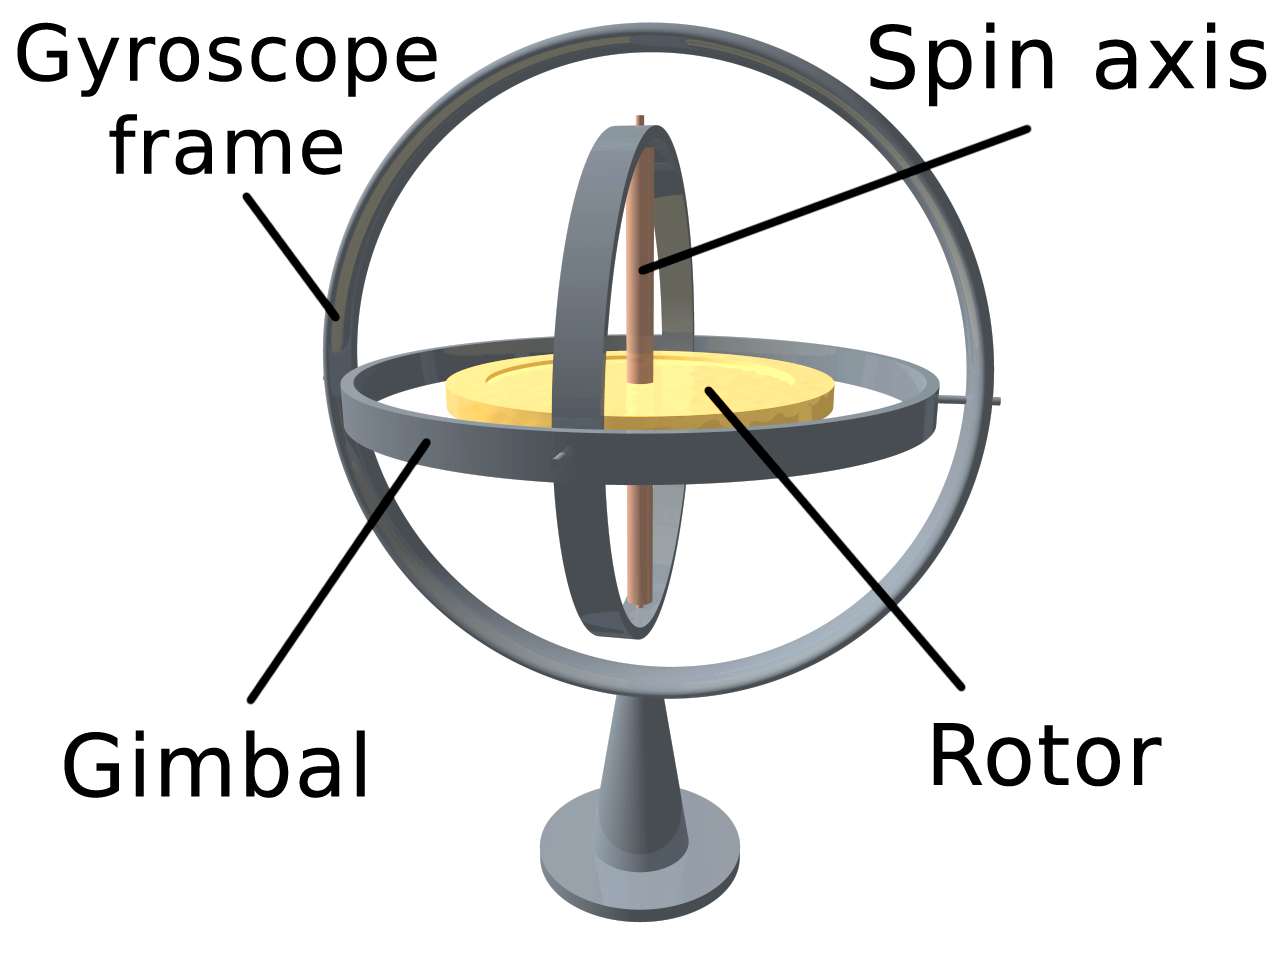
\includegraphics[scale = 0.1]{img/3D_Gyroscope.png}
	    \caption{Composition d'un gyroscope}
	    \label{compositiongyroscope}
	  \end{figure}
	  
	\subsection{Principe}
	  Le gyroscope profite d'un principe physique appelé principe de 
conservation du moment cinétique, ou effet gyroscopique. Cet effet implique que 
lorsqu'on applique une force sur un solide en rotation (le rotor dans notre 
cas), il se crée un couple ($\omega_{p}$) perpendiculaire à cette force. Ce 
couple permet à notre système d'effectuer une rotation autour d'un axe (axe 
défini par un point en contact avec un repère fixe) ce qui a pour effet 
d'annuler la portée instable de la pesanteur. On obtient alors un système en 
rotation parfaitement stable malgré des angles d'inclinaison importants.

	  \begin{figure}[htbp]
	    \centering
	    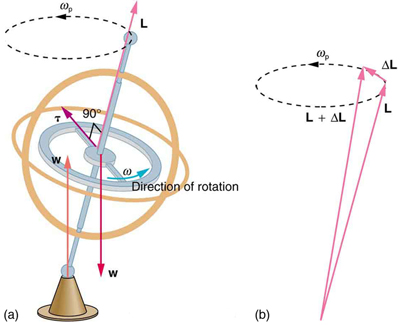
\includegraphics[scale = 1.3]{img/schema_gyro.png}
	    \caption{Descriptif des forces appliquées sur un gyroscope}
	    \label{descriptifforces}
	  \end{figure}
	  
	  \begin{figure}[htbp]
	    \centering
	    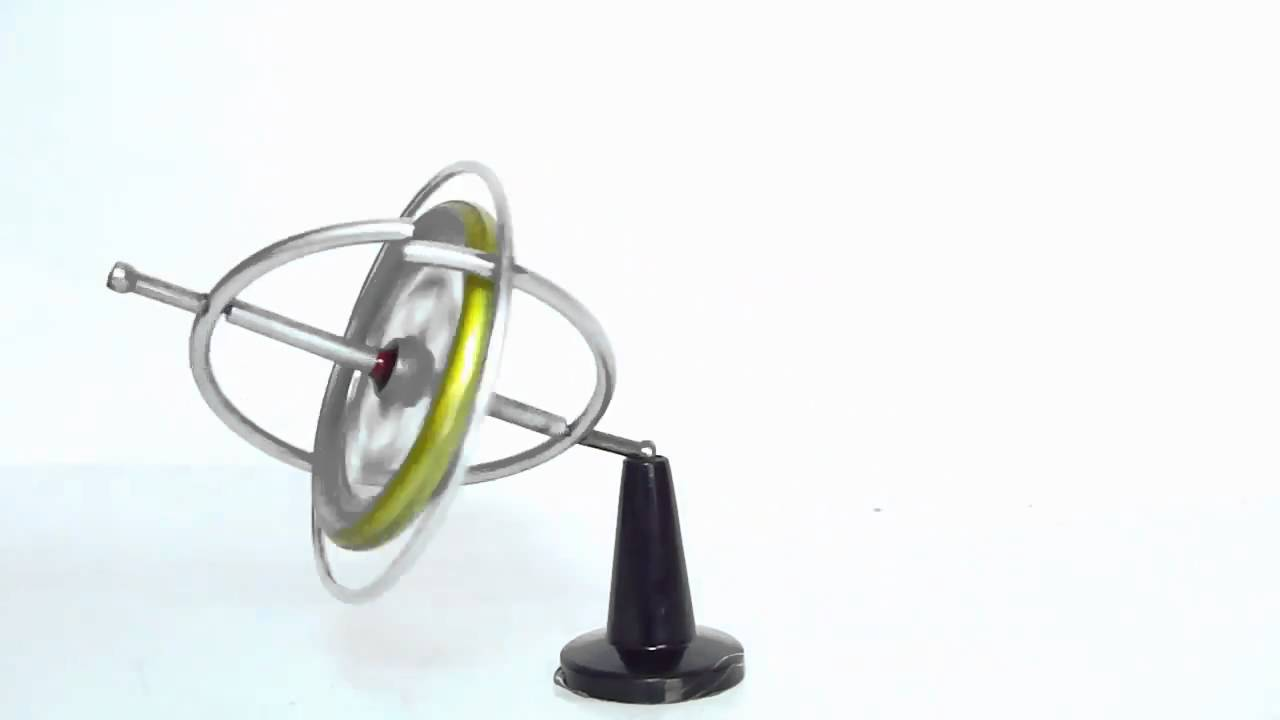
\includegraphics[scale = 0.2]{img/inclinaison.jpg}
	    \caption{Inclinaison maximale}
	    \label{inclinaisonmax}
	  \end{figure}
	  
	  Dans le cas de notre gyroscope, la situation est légèrement 
différente. En effet, si le fonctionnement est le même, notre système est 
inversé. Ainsi, les parties extérieures du gyroscope, fixées à notre drone 
seront mobiles. Elles absorberont les couples et forces énoncées précédemment, 
permettant au rotor de conserver une inclinaison fixe par rapport au repère 
Galiléen.

	  En étudiant les variations d'angles des anneaux extérieurs (puisque 
l'axe du tore central est fixe par rapport au repère terrestre, il est possible 
de connaître la variation d'angle des cadrans) nous sommes en mesure de 
connaître l'orientation de l'appareil par rapport au sol.

	\subsection{Le gyroscope dans notre montage}
	  Le gyroscope choisi pour intégré notre drone est un MPU-6050. Ce type 
de gyroscope, particulièrement répandu dans l'industrie, présente l'avantage 
d'être compatible avec notre montage, relativement abordable financièrement et 
de posséder un accéléromètre. Cet accéléromètre étant destiné à nous fournir 
des informations sur le déplacement, et la position de notre drone. 
 
	  Ce capteur est constitué de trois axes (les axes X et Y étant 
indiqués sur la carte, l'axe Z étant perpendiculaire à la plaque (voir 
Figure \ref{mpu6050schema})). Puisqu'il faut que l'effet gyroscopique puisse 
s'appliquer sur le gyroscope, l'ensemble des angles pouvant être mesurés 
appartiennent à [-80,80]. Passé cette valeur, la gravité serait trop proche de 
la composante créée par l'effet gyroscopique, ce qui fausserait les mesures. 
Les mesures de rotations autour de l'axe Z varient quant à elles entre -180 et 
180.

	  Afin d'utiliser le MPU-6050 dans notre montage, nous nous sommes 
largement inspirés des travaux de Jeff Rowberg\cite{jeffrwork}, qui propose un 
code permettant de mesurer les valeurs obtenues par les capteurs. Fort de ces 
informations, une analyse est effectuée afin de définir l'inclinaison de notre 
drone. Il convient ensuite de piloter les moteurs afin d'effectuer le 
traitement adéquat. Puisque notre drone à pour but de mesurer une topographie, 
il est nécessaire d'obtenir un drone en vol stationnaire, c'est-à-dire 
parallèle au sol. Les moteurs sont donc gouvernés par le gyroscope afin de 
stabiliser l'appareil.

	  \begin{figure}[htbp]
	    \centering
	    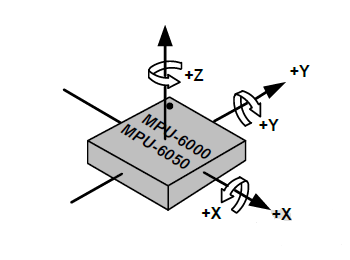
\includegraphics[scale = 0.6]{img/MPU6050_schema.png}
	    \caption{Schéma du MPU-6050}
	    \label{mpu6050schema}
	  \end{figure}
	  
	\subsection{Implémentation}
	  Le programme est divisé en plusieurs parties. Le fichier 
\textit{call\_gyroscope} permet d'appeler les diverses fonctions nécessaires au 
bon fonctionnement du gyroscope. 

	  Les fichiers \textit{I2Cdev.cpp} et \textit{MPU6050.cpp} sont des 
fichiers disponibles sur le compte GitHub de Jeff 
Roswberg\cite{jeff_rowberg_lib}. Ces fichiers permettent la gestion matérielle 
du gyroscope. Ainsi, d'un signal purement électrique et sans grande 
signification, ces bibliothèques permettent d'obtenir des valeurs plus 
intuitives (angles, différentiels de forces, ...).

	  \textit{gyro\_lib} est l'application développée afin d'assurer la 
gestion du gyroscope. Elle est divisée en plusieurs fonctions. La fonction 
\textit{initialise} permet de préparer le gyroscope à la prise de mesure. 
Ainsi, suite à cette fonction, le système est opérationnel pour prendre des 
mesures et les stockera dans les variables \textit{gravity}, \textit{ypr}, 
\textit{aa} et \textit{aaReal} (variables permettant de se rendre 
compte de la valeur de la gravité, de la rotation autour des axes appelés 
\textit{Yaw}, \textit{Pitch} et \textit{Roll}, et de l'accélération). La 
seconde fonction, \textit{loop},  gère la stabilité du drone. Cette fonction 
est appelée lorsque le drone cherche à stabiliser sa position à une position 
particulière. On doit avoir une idée des actions à mener sur les moteurs. Par 
conséquent, lorsqu'elle sera appelée, cette fonction retournera une table de 
cinq entiers, les quatre premiers représentant l'action à effectuer sur un 
moteur (variable \textit{moteur[]}) et le dernier renseignant sur la stabilité 
du drone. Ainsi, si la valeur retournée est positive (respectivement négative), 
il sera nécessaire d'augmenter (respectivement diminuer) la vitesse des 
moteurs. 

	  Pour avoir une idée de l'action à mener sur chaque moteur, on décide 
d'acquérir la valeur des angles d'orientations, grâce aux instructions 
suivantes : 

	  \begin{verbatim}
	    mpu.dmpGetQuaternion(&q, fifoBuffer);
	    mpu.dmpGetGravity(&gravity, &q);
	    mpu.dmpGetYawPitchRoll(ypr, &q, &gravity);
	  \end{verbatim}

	  Puis on évalue la valeur de ces angles en testant :
	  
	  \begin{equation}
	    \frac{ypr[1] * 360}{2*\pi} * \frac{ypr[1] * 360}{2*\pi} * 60
	  \end{equation}

	  Avec $ypr$ une table renvoyant le \textit{YawPitchRoll} (angle 
d'inclinaison) de notre drone. Les facteurs $18$, $M_{PI}$ et $90$ sont des 
facteurs permettant d'obtenir des valeurs en degrés (et non radians). Enfin le 
facteur $60$ permet d'obtenir des actions ayant une influence sur la rotation 
des moteurs. 

	  On peut remarquer que l'action sur les moteurs implique une 
modification coordonnée de différents moteurs. En effet, si le drone est 
incliné avec un $moteur_1$ et un $moteur_4$ trop bas, il sera nécessaire 
d'augmenter sa vitesse de rotation afin qu'il gagne en altitude. Néanmoins, il 
est aussi nécessaire de diminuer la vitesse du $moteur_2$ et du $moteur_3$ afin 
de conserver une altitude plus ou moins stable. La Figure 
\ref{inclinaisondrone} illustre cet exemple.

	  \begin{figure}[htbp]
	    \centering
	    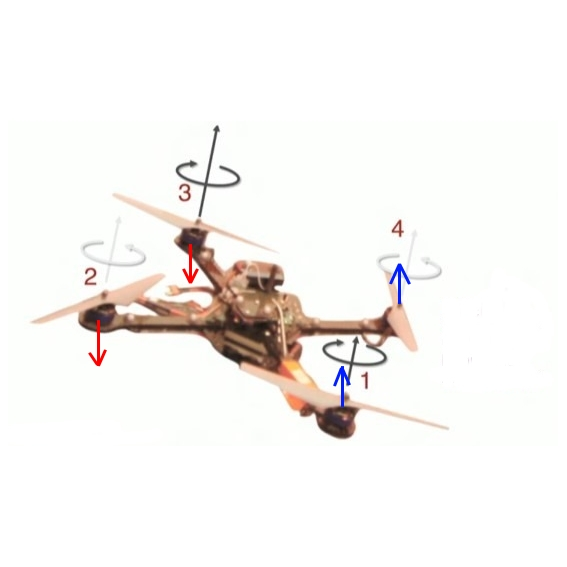
\includegraphics[scale = 0.5]{img/quadcopter.jpg}
	    \caption{Exemple d'action des moteurs suivant l'inclinaison du 
drone}
	    \label{inclinaisondrone}
	  \end{figure}

	  En évaluant la valeur de \textit{ypr}, on est en mesure de connaître 
l'inclinaison du drone afin de réévaluer la vitesse des bons moteurs. Une fois 
ceci effectué, on peut renvoyer notre table à l'Arduino qui n'aura alors qu'à 
modifier la vitesse des moteurs
    
    \chapter{Calculs mécaniques et électriques}
      \section{Théorie physique pour le calcul de la puissance requise par les 
moteurs}
	Afin de choisir correctement les moteurs, il est nécessaire de 
connaître la fonction $Puissance = f(Poids)$, soit la relation entre la 
puissance fournie par les moteurs et le poids qu'ils permettent de porter. Pour 
déterminer cette relation, on va considérer notre sytème comme un système 
isolé (c'est-à-dire sans interactions avec l'extérieur). Il est formé par 
trois parties, une partie centrale constituée de la pale, une inférieure 
permettant à l'air d'entrer dans la pale et une partie supérieure lui 
permettant d'en sortir. 

	  \begin{figure}[htbp]
	    \centering
	    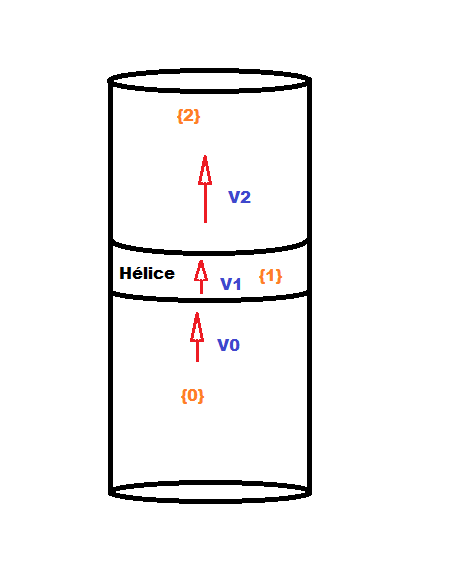
\includegraphics[scale = 0.5]{img/systeme_isole.png}
	    \caption{Schéma d'un système isolé}
	    \label{systemisole}
	  \end{figure}
	  
	Chaque partie a une pression particulière, ce qui a pour conséquence 
d'appliquer une force sur les pales. On peut exprimer ces forces par l'équation 
\ref{eq:forcepal}.

	\begin{equation}
	  \label{eq:forcepal}
	  F(Pression) = Pression * Surface 
	\end{equation}

	Cette force étant dirigée vers les pales, il se crée deux forces de 
directions opposées et donc un différentiel de force $F_{diff}$ tel que donné 
par l'équation \ref{eq:fdiff}.

	\begin{equation}
	  \label{eq:fdiff}
	  F_{diff}(Pression) = (Pression_{haut} - Pression_{bas}) * Surface
	\end{equation}

	Donc, du fait de la rotation des pales, il se crée une différence de 
pression, ce qui a pour conséquence de favoriser la création d'une force. 
Il est courant d'appeler des différences de force, \textit{sustentation}.

	Maintenant que l'on est en mesure de comprendre le principe de 
sustentation, il est nécessaire de l'estimer afin de connaître la 
puissance à fournir pour que le drone puisse décoller. 

	Considérons le débit de l'air ($Q$) :
	
	\begin{equation}
	  \label{eq:debit}
	  Q = \rho * Surface * Vitesse
	\end{equation}
	
	avec :
	
	\begin{itemize}
	  \item $\rho$ : masse volumique de l'air
	  \item Surface : surface sur la portion considérée
	  \item Vitesse : vitesse moyenne de l'air dans cette portion
	\end{itemize}
	
	On peut exprimer la puissance du rotor par l'équation 
\ref{eq:puissancerotor}.
	
	\begin{equation}
	  \label{eq:puissancerotor}
	  P_{r} = F_{n} * V_{1} 
	\end{equation}
	
	En utilisant le théorème de la quantité de 
mouvement\cite{thquantmouvement}, on obtient l'équation 
\ref{eq:quantitemouvement}:

	\begin{equation}
	  \label{eq:quantitemouvement}
	  \Sigma(quantit\acute{e}s \ de \ mouvement) = \Sigma (forces \ 
ext\acute{e}rieures) 
	\end{equation}
	
	Soit,
	
	\begin{equation}
	  \label{eq:force}
	  F_{n} = Q * V_{2} - Q * V_{0} 
	\end{equation}
	
	Afin de simplifier nos calculs, nous devons considérer certaines 
hypothèses. Ainsi, au sein du conduit, on peut négliger les échanges avec 
l'extérieur (système fermé). Par conséquent, on peut utiliser la relation de 
Bernouilli, soit :

	\begin{equation}
	  \label{eq:cinetique}
	  E_{c} = \frac{1}{2} * \rho * V^{2} 
	\end{equation}
	
	Si le système est considéré comme fermé, alors on peut en déduire que la 
puissance utilisée se dissipe sous forme d'énergie cinétique. Pour le système 
(rotor + pale), les seuls échanges possibles sont donc ceux avec les systèmes à 
ses extrémités ({0} et {1}, voir figure \ref{systemisole}). On a donc :

	\begin{equation}
	  d_{Puissance} = (E_{c_{2}} - E_{c_{0}}) * d_{Surface}
	\end{equation}

	d'où en utilisant l'équation \ref{eq:cinetique}:
	
	\begin{equation}
	  d_{Puissance} = \frac{1}{2} * \rho * (V_{2}^{2} - V_{0}^{2}) * 
d_{Surface}
	\end{equation}
	
	Soit l'équation de la puissance :
	
	\begin{equation}
	  \label{eq:puissance}
	  Puissance = \frac{1}{2} * Q(V_{2}^{2}-V_{0}^{2}) 
	\end{equation}
	
	or d'après l'équation \ref{eq:puissancerotor} et en remplaçant 
$F_{n}$, par l'équation \ref{eq:force} on obtient : 
	
	\begin{equation}
	  \label{eq:puissance2}
	  P_{r} = Q(V_{2}-V_{0})*V_{1} 
	\end{equation}
	
	À partir des équations \ref{eq:puissance} et \ref{eq:puissance2}, on 
peut établir l'équation suivante : 
	
	\begin{equation}
	  Q(V_{2} - V_{0})*V_{1} = \frac{1}{2} * Q (V_{2}^{2}-V_{0}^{2})
	\end{equation}
	
	Soit :
	\begin{equation}
	  \label{eq:vitessePale}
	  V_{1} = \frac{(V_{2} + V_{0})}{2} 
	\end{equation}
	
	on a alors :
	
	\begin{equation}
	  V_{2} = 2*(V_{1} - V_{0})
	\end{equation}
	
	de plus, d'après \ref{eq:force}, en remplaçant $V_{2}$ par 
\ref{eq:vitessePale} on a :
	
	\begin{equation}
	  F_{n} = Q(2V_{1} - 2V_{0})
	\end{equation}
	
	En utilisant \ref{eq:debit}, on obtient :
	
	\begin{equation}
	  Fn = 2 \rho * Surface * V_{1} * (V_{1} - V_{0})
	\end{equation}

	d'où :
	
	\begin{equation}
	  \label{eqForce}
	  F_{n} =  2 \rho * Surface *V_{1} * V_{f}
	\end{equation}
	
	avec $V_{f} = V_{1} - V_{0}$, la vitesse finale.
	
	Il est a noter qu'au décollage, on a $V_{0} = 0$, donc :
	
	\begin{equation}
	  \label{eq:decollage}
	  F_{n} =  2 \rho * Surface * V_{1}^{2}
	\end{equation}
	
	Enfin d'après \ref{eq:puissance1} on a :
	
	\begin{equation}
	  V_{1} =  \frac{P_{r}}{F_{n}}
	\end{equation}
	
	donc, d'après \ref{eq:decollage} :
	
	\begin{equation}
	  F_{n} = 2 \rho * Surface * (\frac{P_{r}}{F_{n}})^{2}
	\end{equation}
	
	ce qui revient à :
	
	\begin{equation}
	  \label{eq:forceoutput}
	  F_{n}^{3} = 2 \rho * Surface * P_{r}^{2}
	\end{equation}
	
	avec :
	
	\begin{itemize}
	  \item $F_{n}$ : force émise par la pale
	  \item $\rho$ : masse volumique de l'air ($= 1,225kg.m^{-3}$)
	  \item $S = \frac{\pi * {D}^{2}}{4}$, avec $D$ le diamètre des pales
	\end{itemize}
	
	Dans le cadre de notre drone, on désire que la force des pales soit 
supérieure au poids du drone. Donc :

	\begin{equation}
	  F_{n}(total) > \Sigma (forces \ verticales) 
	\end{equation}
	
	On suppose que chaque rotor fournit la même puissance, soit :
	
	\begin{equation}
	  F_{n}(total) = 4 * F_{n} 
	\end{equation}

	De plus, la seule force verticale étant le poids, on a : 
	\begin{equation}
	  \Sigma (forces \ verticales) = m * g
	\end{equation}
	
	avec :
	
	\begin{itemize}
	  \item  m : masse totale du drone
	  \item  g = valeur du champ de la pesanteur ($=9,81m.s^{-2}$
	\end{itemize}

	Donc, à l'aide de l'équation \ref{eq:forceoutput}, on a : 
	
	\begin{equation}
	  4 * \sqrt[3]{2 \rho * Surface * P_{r}^{2}} > m*g
	\end{equation}
	
	D'où l'équation finale \ref{eq:finale}:
	
	\begin{equation}
	  \label{eq:finale}
	  P_{r}  > \sqrt[2]{\frac{\frac{m*g}{4}^{3}}{2 \rho * Surface}}
	\end{equation}
	
      \section{Calcul de l'autonomie de la batterie}
	L'autonomie de la batterie peut être connue à partir de la capacité de 
celle-ci et de la consommation électrique de chaque composant :

	\begin{equation}
	  autonomie = \frac{capacit\acute{e}}{(consommation_{moteur} * 4) + 
consommation_{autres}} * 60
	\end{equation}
	
	avec :
	
	\begin{itemize}
	  \item $capacit\acute{e}$ : la capacité de la batterie (en mAh)
	  \item $consommation_{moteur}$ : la consommation électrique (en mA) 
d'un moteur pour fournir la puissance $P_{r}$ requise pour le décollage (voir 
\ref{eq:finale})
	  \item $consommation_{autres}$ : la consommation électrique (en mA) 
des autres composants
	  \item un taux d'efficacité de 60\%
	\end{itemize}
	
	La consommation électrique d'un moteur pour fournir la puissance 
$P_{r}$ peut être calculée par l'équation suivante :

	\begin{equation}
	  consommation_{moteur} = \frac{P_{r}}{tension * taux \ 
d'\acute{e}fficatit\acute{e}_{moteur}}*1000
	\end{equation}

      \section{Pratique}
	Grâce à la théorie, nous sommes en mesure de déterminer si un drone 
peut voler ou non. Il est maintenant nécessaire de créer les outils permettant 
d'exploiter ces calculs. 

	On pourra remarquer que sur l'équation \ref{eq:finale}, les valeurs 
caractéristiques de notre système sont :
	\begin{itemize}
	  \item $m$ : la masse de notre drone
	  \item $Surface$ : la surface d'action des pales
	  \item $Pr$ : la puissance générée par chaque moteur
	\end{itemize}
	
	Nous avons donc créé un calculateur permettant de nous indiquer si 
notre drone serait en mesure de décoller ou non (voir section 
\ref{sec:calculateur}). 

	  \begin{figure}[htbp]
	    \centering
	    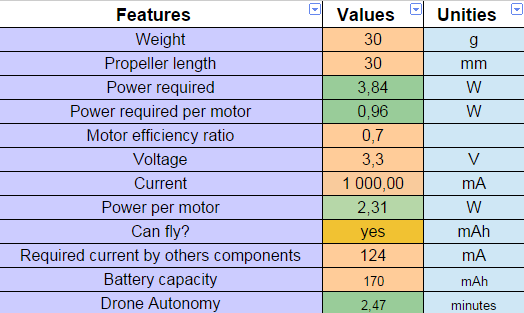
\includegraphics[scale = 0.5]{img/calculateur.png}
	    \caption{Exemple d'utilisation du calculateur}
	    \label{calculateur}
	  \end{figure}

	Sur la figure \ref{calculateur}, on peut remarquer que notre 
calculateur nous permet de renseigner certaines valeurs telles que le poids du 
drone (nécessaire pour avoir $m$), mais aussi la taille des pales afin de 
connaître leur surface d'action. À partir de ces informations on est en mesure 
de calculer la puissance nécessaire par moteurs. On recueille ensuite les 
informations sur les moteurs (courants, tension, facteur d'efficacité). 
Notre drone sera alors en mesure de voler si :

	\begin{equation}
	  Power \ per \ motor > Power \ required \ per \ motor 
	\end{equation}

	Des informations telles que l'autonomie peuvent être obtenues en 
renseignant les champs relatifs aux autres composants.

  \listoffigures
  
  \raggedright
  \bibliographystyle{unsrt}
  \bibliography{biblio}
\end{document}